\documentclass[thesis=M,english,hidelinks]{FITthesis}[2012/10/20]

\usepackage[utf8]{inputenc} % LaTeX source encoded as UTF-8

\usepackage{graphicx} % graphics files inclusion
\usepackage{subfig}
\usepackage{amsmath}
\usepackage{amssymb}
\usepackage{relsize}
\usepackage{textcomp}
\usepackage[dvipsnames]{xcolor}
\usepackage[binary-units=true]{siunitx}

\usepackage{pgfplots}
\usepackage{pgfplotstable}
\pgfplotsset{compat=1.8}

\usepackage{amsthm}
\theoremstyle{definition}
\newtheorem{definition}{Definition}
\newtheorem{theorem}{Theorem}
\newtheorem{lemma}{Lemma}
\newtheorem{example}{Example}
\usepackage{float}

\usepackage{algorithm}
\usepackage[noend]{algpseudocode}

\usepackage{tikz}
\usetikzlibrary{shapes}
\usetikzlibrary{arrows.meta}
%\tikzset{every node/.style={draw}}

\usepackage{xspace}
\newcommand{\PC}{\textbf{P}\xspace}
\newcommand{\NP}{\textbf{NP}\xspace}
\newcommand{\NPH}{\textbf{NP}-hard\xspace}
\newcommand{\NPC}{\textbf{NP}-complete\xspace}

% table struts
\newcommand\Tstrut{\rule{0pt}{2.6ex}}       % Top strut
\newcommand\Bstrut{\rule[-1.2ex]{0pt}{0pt}} % Bottom strut

% table footnotes
\usepackage{threeparttable}
\usepackage{etoolbox}
\appto\TPTnoteSettings{\footnotesize}

\usepackage{dirtree}

\department{Department of Theoretical Computer Science}
\title{Parameterized Algorithms for Steiner Trees}
\authorGN{Peter}
\authorFN{Mitura}
\author{Peter Mitura}
\authorWithDegrees{Bc. Peter Mitura}
\supervisor{RNDr. Ondřej Suchý, Ph.D.}

\acknowledgements{
    First and foremost, I would like to thank my supervisor RNDr. Ondřej Suchý, Ph.D. for his thorough and insightful
    advice and great amounts of help provided throughout the whole creation process. A big thank you also goes to my
    girlfriend and family for they immense support and patience.

    I also want to express my gratitude to all members of the FIT Ducklings competitive programming team (both in its
    2016 and 2017 roster) and people around the ACM training sessions on FIT CTU, who have shown me that all you
    ever need is to use binary search and you will get OK. To people that participated on the organization of the
    Algorithms and Graphs 1 course, and to those who somehow suffered through my classes. To the organization team of
    the FIKS correspondence seminar, for all those wonderful camps filled with games, hikes, and problem solving I could
    co-organize with them.
    
    And last but not least, to Tomáš Valla and Ondřej Suchý for making all of the above possible, and organizing the
    great Theoretical seminar and the STIGMA school.

    My studies were as awesome as they were thanks to all of you.
}

\abstractEN{
    Given a weighted graph and a subset of its vertices called terminals, the \textsc{Steiner Tree} problem is to find
    its connected subgraph of the minimum weight, that contains all of the given terminals. This problem is widely known
    to be \NPH, and has a wide range of applications in integrated circuit design, networking, transportation and more.
    In our thesis, we analyze Dreyfus-Wagner, Erickson-Monma-Veinott, and Nederlof algorithms for this problem
    parameterized by the number of vertices, and the rank-based dynamic programming algorithm for the problem
    parameterized by treewidth. For all of these algorithms, we provide an optimized implementation, and compare it with
    other solutions by submitting our results to the PACE 2018 challenge.
}
\abstractCS{
    Je-li dán vážený graf a podmnožina jeho vrcholů zvaných terminály, problém Steinerova stromu spočívá v nalezení
    souvislého podgrafu s nejmenší váhou, který obsahuje všechny terminály. Jedná se o známý \textbf{NP}-těžký problém,
    který nalézá užití kupříkladu v návrhu integrovaných obvodů, nebo počítačových a dopravných sítích. V této práci
    rozebereme algoritmus od Dreyfuse a Wagnera, od Ericksona, Monmy a Veinotta, a Nederlofův algoritmus, které řeší
    verzi tohoto pro\-blé\-mu parametrizovanou počtem terminálů, a algoritmus využívající dynamické programování a
    matici řezů pro parametrizaci dle stromové šířky.  Pro všechny popsané algoritmy vytvoříme optimalizovanou
    implementaci a pro porovnání s jinými řešeními ukážeme její výsledky v soutěži PACE 2018.
}
\placeForDeclarationOfAuthenticity{Prague}
\keywordsCS{Steinerovy stromy, Parametrizované algoritmy, optimalizace, stromová šírka, grafové algoritmy}
\keywordsEN{Steiner tree, parameterized algorithms, optimization, treewidth, graph algorithms}
\declarationOfAuthenticityOption{4} %select as appropriate, according to the desired license (integer 1-6)


\begin{document}

\setsecnumdepth{part}
\chapter{Introduction}

Finding the Steiner tree is a well known problem, that generally finds the cheapest way to connect a set of
objects called terminals. It can be formalized in many settings, including various metric spaces and graph types. In
our thesis, we will use a version defined on undirected weighted graphs, which is arguably the most common formulation
of this problem.

Its optimization variant is also one of the oldest known \NPH problems \cite{Karp1972}, implying we can presumably only
solve it in superpolynomial time. As finding the Steiner tree has many applications in circuit design and networking,
there is an incentive to create an efficient solution for this problem, that could process inputs with more than just a
few dozens of vertices.

Parameterization is a technique applicable in such cases, allowing us to find algorithms for \NPH problems that are
polynomial in the input size, but exponential in some other measure of the input, called the parameter. We will mainly
consider two kinds of parameters in this thesis, the number of terminals and a measure of graph called treewidth, which
can be intuitively described as the similarity of a graph to a tree.

Our work focuses on implementing known algorithms for these kinds of parameterization as efficiently as possible.  For
parameterization by number of terminals, we have looked into Dreyfus-Wagner \cite{Dreyfus1971} dynamic programming
algorithm, its improved version known as the Erickson-Monma-Veinott algorithm \cite{Erickson1987}, and a newer algorithm
presented by Nederlof in 2013 \cite{Nederlof2013}, utilizing the inclusion-exclusion principle.

In case of parameterization by treewidth, we have implemented the classical dynamic programming algorithm, augmented
with the rank-based table reduction, as described by Bodlaender et al. in \cite{Bodlaender2012}.

As an additional motivation for solving this problem, an international parameterized algorithm competition known as
PACE had the Steiner tree problem as its main topic for year 2018 \cite{PaceReport}, allowing us to submit our
implementation and compare it with solutions from all over the world.

% -----------------------------------------------------------------------------

\setsecnumdepth{all}
\chapter{Basic concepts}

In this chapter, we will introduce the theory that is essential for the algorithms we discuss in the remaining chapters of
this thesis. Most definitions are laid out in a similar way as they appear in FIT CTU courses, namely MI-CPX, MI-PAM and
BI-AG1. Some definitions in Section \ref{sec:complexity} presume basic knowledge of terms used in formal language
theory, as seen in \cite[p. 11]{Melichar2013}.

\section{Graph theory}

We will start by defining standard graph theory concepts that will be used in the problem definition, and algorithm
descriptions throughout this work. 

\begin{definition}
    A \emph{graph} is an ordered pair $(V, E)$. $V$ is a set of its \emph{vertices} and $E$ is a set of
    its \emph{edges}, where each edge is an unordered pair of distinct vertices from $V$. Given a graph $G$, we will
    denote its set of vertices as $V(G)$, and its set of edges as $E(G)$.
\end{definition}

\begin{definition}
    Graph $H$ is \emph{subgraph} of graph $G$ (denoted $H \subseteq G$) when it holds that $V(H) \subseteq V(G)$ and
    $E(H) \subseteq E(G)$.
\end{definition}

\begin{definition}
    Graph $H$ is an \emph{induced subgraph} of graph $G$ when it holds that $V(H) \subseteq V(G)$ and
    $E(H) = \{\{u, v\} \mid \{u, v\} \in E(G) \land u, v \in V(H)\}$. We denote an induced subgraph of $G$ defined by a
    vertex set $X \subseteq V(G)$ as $G[X]$.
\end{definition}

\begin{definition}
    A \emph{path} of length $n \geq 0, n \in \mathbb{N}$ is a graph $P_n$ such that:
    $$
    P_n = (\{0, \ldots, n\}, \{\{i, i+1\}\ |\ i \in \{0, \ldots, n-1\}\}).
    $$
    The vertices $0$ and $n$ are called the \emph{endpoints} of the path. We say that there is a path in a graph $G$
    between vertices $u, v \in V(G)$, when there is a subgraph of $G$ that is a path and has vertices $u$ and $v$ as
    its endpoints. A path in graph $G$ is called the \emph{shortest path} between vertices $u$ and $v$, if there is no
    shorter path between $u$ and $v$ in $G$. By $dist(u, v)$, we will denote the length of the shortest path between
    vertices $u$ and $v$ in $G$.
\end{definition}

\begin{definition}
    A \emph{cycle} of length $n \geq 3, n \in \mathbb{N}$ is a graph $C_n$ such that:
    $$
    C_n = (\{1, \ldots, n\}, \{\{i, i+1\}\ |\ i \in \{1, \ldots, n-1\}\} \cup \{n, 1\}).
    $$
\end{definition}

\begin{definition}
    Graph $G$ is \emph{connected}, if there is a path in $G$ between each pair of vertices in $V(G)$.
\end{definition}

\begin{definition}
    We call an induced subgraph $H$ of $G$ a \emph{connected component} (or just \emph{component}) of $G$ if $H$ is
    connected, and there is no connected subgraph $F$ of $G$, such that $H$ is a subgraph of $F$ and $H \neq F$.
\end{definition}

\begin{definition}
    A \emph{tree} is a connected graph that does not contain a cycle as a subgraph.
\end{definition}

\begin{definition}
    An \emph{oriented graph} is an ordered pair $(V, E)$. $V$ is again a set of its vertices and $E$ is a set of
    its edges, but each edge is an \emph{ordered} pair of distinct vertices from $V$. For each edge $(u, v) \in E$, we
    say that $u$ is a \emph{parent} of v and $v$ is a \emph{child} of $u$.
\end{definition}

\begin{definition}
    A \emph{rooted tree} is an oriented graph $R$ created from a tree~$T$, where one of the vertices $r \in V(T)$ is
    chosen to be the \emph{root}, and $R = (V(T), \{(u, v) \mid \{u, v\} \in E(T) \land dist(r, u) < dist(r, v)\})$.
\end{definition}

\section{Complexity}
\label{sec:complexity}

As the time performance of analyzed algorithms is one of our main concerns, we will use standard complexity classes to
classify the solved problem in the polynomial hierarchy. First, we will formally define a problem, and an algorithm that
solves it:

\begin{definition}
    A \emph{problem} is a formal language $P \subseteq \Sigma^*$, where $\Sigma$ is a finite alphabet. We say
    that an algorithm solves problem $P$ if it decides for every instance $w \in \Sigma^*$ whether it belongs
    to $P$ in finite time.
\end{definition}

\begin{definition}
    \PC denotes the class of all problems that can be solved by a deterministic algorithm running in polynomial
    time.
\end{definition}

\begin{definition}
    \NP denotes the class of all problems, such that their solution is of polynomial size and can be verified by a
    deterministic algorithm running in a polynomial time.
\end{definition}

\begin{theorem}
    $\PC \subseteq \NP$
\end{theorem}

\begin{proof}
    Consider a solution to any problem $P \in \PC$. We can verify it in polynomial time by running the
    algorithm that solves $P$ (which has to exist because it belongs to \PC) and comparing the results.
\end{proof}

It is also widely presumed that $\PC \neq \NP$, meaning there are problems that can be verified in polynomial time,
but solved only in superpolynomial time.

\begin{definition}
    A \emph{polynomial-time reduction} of a problem $P$ to a problem $\mathcal{Q}$ is a function $f:\ \Sigma^*
    \rightarrow \Sigma^*$, that can be computed in polynomial time, and
    $$
    (\forall w \in \Sigma^*)\ w \in P \Leftrightarrow f(w) \in \mathcal{Q}
    $$
    If such a reduction exists, we say that $P$ can be polynomially reduced to $\mathcal{Q}$ and denote it as
    $P \lhd \mathcal{Q}$.
\end{definition}

\begin{definition}
    A problem $\mathcal{H}$ is \NPH if it holds that
    $$
    (\forall P \in \textbf{NP})\ P \lhd \mathcal{H}
    $$
\end{definition}

\begin{definition}
    We say that problem $P$ is \NPC if
    $$
    P \in \textrm{\textbf{NP}-hard}\,\cap\,\NP
    $$
\end{definition}

Even though there is a presumption that \PC $\neq$ \NP holds, there are techniques that can make the computation
times for \NPH problems on bigger instances feasible under certain conditions.

Parameterization is one of such possibilities. Its basic idea is to consider some property of the input other than size,
and create an algorithm that runs in exponential time depending on this property, but only polynomial time with respect
to the input size.

This does not provide a universal solution to large inputs, we still expect that the algorithm time complexity will be
exponential in input size for some parameter values unless \PC = \NP.

However, this technique still allows us to solve large classes of instances we could not approach with a
non-parameterized algorithm.

\begin{definition}
    A \emph{parameterized problem} is a formal language $\mathcal{L} \subseteq \Sigma^* \times \mathbb{N}$, where $\Sigma$ is
    a finite alphabet, and the integer part is called the \emph{parameter}.
\end{definition}

\begin{definition}
    Parameterized problem $L$ is \emph{fixed-parameter tractable}, if there is an algorithm that decides, whether $(X, k)
    \in \mathcal{L}$ in time $f(k) \cdot \lvert X \rvert^c$, where $f$ is any function with a single integer parameter,
    and $c$ is a constant. Such solution is called a \emph{parameterized algorithm} or \emph{FPT algorithm}, and a class
    of all fixed-parameter tractable problems is called \textbf{FPT}.
\end{definition}

Throughout this thesis, we will use the common form of the $\mathcal{O}$-notation to express asymptotic complexity:

\begin{definition}
    Let $f(n)$ and $g(n)$ be finite and positive functions. We than say, that $g(n)$ is an \emph{asymptotic upper bound}
    of $g(n)$ (denoted $f(n) = \mathcal{O}(g(n))$) if

    $$
    (\exists c \in \mathbb{R}^+)\,(\exists n_0 \in \mathbb{N}^+)\,(\forall n \geq n_0)\ f(n) \leq c \cdot g(n)
    $$
\end{definition}

While discussing time complexity of a parameterized algorithm, we would occasionally use the $\mathcal{O}^*$ notation that
leaves out polynomial factors. Formally:

\begin{definition}
    Consider a parameterized algorithm deciding if $(X, k) \in L$ with time complexity of $f(k) \cdot \lvert X
    \rvert^c$. We can then denote its complexity as $\mathcal{O}^*(f(k))$.
\end{definition}

\section{Steiner tree problem}

The Steiner tree problem can be formulated as a decision, or an optimization problem. When formally defining it, we will
only consider the latter variant, as it directly stems from the decision formulation, and it will be the one we will be
solving. Furthermore, we will start by introducing the simpler, unweighted version of this problem:

\begin{definition}
    (\textsc{Unweighted Steiner Tree Problem}): We are given a graph $G = (V, E)$ and a subset of its vertices $K
    \subseteq V$ called \emph{terminals}. The problem is to find a connected subgraph $T$ of $G$, such that it contains
    all vertices in $K$, and the number of its edges is minimal.
\end{definition}

It can be easily shown that the solution of any \textsc{Unweighted Steiner Tree Problem} instance is a tree. By
contradiction, if there was a solution that was not a tree, we could take any of its spanning trees, and it would be a
subgraph that fulfills all conditions, but contains less edges.

We will continue with a common extension of this problem that uses weighted edges, which is also the main focus of this
work:

\begin{definition}
    (\textsc{Steiner Tree} problem): Given a graph $G = (V, E)$, a function $w: E \rightarrow \mathbb{N}$ assigning
    an integer weight to every edge, and a subset of its vertices $K \subseteq V$
    as an input, the problem is to find a connected subgraph $T$ of $G$, such that it contains all vertices in $K$, and
    the sum of its edge weights is minimal.
\end{definition}

The decision unweighted version was shown to be \NPC by Karp in 1972 \cite{Karp1972} as one of his original 21 \NPC problems.

This naturally extends to the optimization variants being \NPH. The same classifications also apply to the weighted
versions of the problem.

\section{Partitions}

Throughout some of the dynamic programming solutions to the \textsc{Steiner Tree} problem, we will often need a way to
describe connected components of a partial solution to a given problem instance. In order to do this, we will use the
notion of partitions, defined as follows:

\begin{definition}
    For a given set of graph vertices $U$, a \emph{partition} $P$ of $U$ is a set of $n \in \mathbb{N}_0$ sets $\{c_1, \ldots,
    c_n\}$, where $(\forall i \in \mathbb{N}, 1 \leq i \leq n)\ \emptyset \neq c_i \subseteq U$, such that
    $$
    (c_1 \cup c_2 \cup \ldots \cup c_n = U) \land ((\forall i, j \in \mathbb{N}, 1 \leq i, j \leq n, i \neq j)\,c_i \cap c_j = \emptyset).
    $$
\end{definition}

As we are going to use partitions exclusively for graph purposes, we only define them for vertex sets (as opposed to
standard partitions, which can be used over any set). Following the graph terminology, we will also refer to elements of
a partition as \emph{components}.

Since the partitions will help us describe subproblems, it is natural that in the process of combining their solutions,
we also want to merge their corresponding partitions. To do this, we will formalize the partition merging:

\begin{definition}
    Let $P_1$ and $P_2$ be partitions of a vertex set $U$. We will define the \emph{merge} of these partitions, denoted
    $P_1 \sqcup P_2$, as a partition $M$ of $U$, such that for each pair of elements $u, v \in U$, it holds that $u$
    and $v$ will be in the same component within $M$ if and only if there is a sequence of vertex pairs $(u, v_1), (v_1,
    v_2), \ldots, (v_{p-1}, v_p), (v_p, v)$, such that $p \geq 0$ and for each pair in this sequence, both elements of
    the pair belong to the same component within $P_1$ or $P_2$.
\end{definition}

Additionally, we can constraint this notion to only include merges without redundant connectivity:

\begin{definition}
    We say that a merge of partitions $P_1$ and $P_2$ of a vertex set $U$ is \emph{acyclic}, if there is no pair of
    vertices $u, v \in U, u \neq v$, that would belong to the same component within $P_1$ and $P_2$ at the same time.
\end{definition}

Note that the term \emph{acyclic} is derived from an intuition, where we perform the merge by representing partitions as
two separate graphs, and connecting all pairs of vertices with a matching label, as demonstrated in Figure
\ref{fig:cyclicmerge}.

\begin{figure}
    \centering
    \tikz[every node/.style={draw, minimum size=0.8cm}] {
        \node (a1) at (0,   1.5) [circle] {$a_1$};
        \node (b1) at (1.5, 1.5) [circle] {$b_1$};
        \node (c1) at (3,   1.5) [circle] {$c_1$};
        \node (d1) at (4.5, 1.5) [circle] {$d_1$};
        \node (e1) at (6,   1.5) [circle] {$e_1$};
        \node (f1) at (7.5, 1.5) [circle] {$f_1$};
        \node (g1) at (9,   1.5) [circle] {$g_1$};

        \draw (a1) edge[-] (b1)
              (b1) edge[-] (c1)
              (d1) edge[-] (e1);

        \node (a2) at (0,   0) [circle] {$a_2$};
        \node (b2) at (1.5, 0) [circle] {$b_2$};
        \node (c2) at (3,   0) [circle] {$c_2$};
        \node (d2) at (4.5, 0) [circle] {$d_2$};
        \node (e2) at (6,   0) [circle] {$e_2$};
        \node (f2) at (7.5, 0) [circle] {$f_2$};
        \node (g2) at (9,   0) [circle] {$g_2$};

        \draw (b2) edge[-] (c2)
              (c2) edge[-] (d2)
              (f2) edge[-] (g2);

        \draw (a1) edge[-] (a2)
              (b1) edge[-] (b2)
              (c1) edge[-] (c2)
              (d1) edge[-] (d2)
              (e1) edge[-] (e2)
              (f1) edge[-] (f2)
              (g1) edge[-] (g2);
    }
    \caption{Merge of partitions $\{\{a, b, c\}, \{d, e\}, \{f\}, \{g\}\}$ and
    $\{\{a\}, \{b, c, d\}, \allowbreak \{e\}, \{f, g\}\}$, which is not acyclic because of vertices $b$ and $c$.}
    \label{fig:cyclicmerge}
\end{figure}

This intuition may not directly translate into our usage of partitions later on; for instance, we will use them to
represent components through their representatives in some small subset of the whole graph. Even in this case though, if
a merge is not acyclic, it would mean that one of the partitions brings some redundant connectivity, and we could get
the same merge result by using less edges somewhere within its solution.

% -----------------------------------------------------------------------------

\chapter{Parameterization by the number of terminals}

Using the size of the set of terminals $K$ in \textsc{Steiner Tree} problem as a parameter is likely the oldest and most
used way of parameterizing this problem. In the following descriptions, let us denote the number of vertices in the input
graph $G = (V, E)$ as $n$, the number of edges as $m$ and the size of the terminal set as $k$.

The first algorithm that uses a parameter $k$ was introduced in 1971 by Dreyfus and Wagner \cite{Dreyfus1971} with a
time complexity of $\mathcal{O}^*(3^k)$, and this result had not been improved until 1987.  A brief history of results for
parameterization in number of terminals is shown in Table \ref{tab:terminals}, and we will give detailed description for
chosen algorithms in this chapter.

\begin{table}[htb]
    \centering
    \begin{threeparttable}[b]
        \caption{Overview of results in parameterized \textsc{Steiner Tree} problem with $k$ as a parameter.}
        \label{tab:terminals}

        \bgroup
        \def\arraystretch{1.5}
        \begin{tabular}{ p{1cm}  p{5cm}  p{3.5cm}  p{1.5cm} }
            \textbf{Year} & \textbf{Authors} & \textbf{Time complexity} & \textbf{Citations} \\ \hline \Bstrut
            1971 & S. E. Dreyfus, R. A. Wagner & $\mathcal{O}(3^k n + 2^k n^2 + \newline n(m + n \log n)$ &
            \cite{Dreyfus1971}
            \\
            1987 & R. E. Erickson, C. L. Monma, A. F. Veinott & $\mathcal{O}(3^k n + \newline 2^k (m + n \log n))$ &
            \cite{Erickson1987}
            \\
            2006\tnote{1} & B. Fuchs, W. Kern, X. Wang & $\mathcal{O}^*(2.684^k)$ & \cite{Fuchs2007}
            \\
            2006 & D. M{\"o}lle, Daniel, S. Richter, P. Rossmanith & $\mathcal{O}^*((2+\epsilon)^k), \epsilon > 0$ &
            \cite{Molle2006}
            \\
            2007\tnote{2} & A. Bj\"{o}rklund, T. Husfeldt, P. Kaski, M. Koivisto & $\mathcal{O}^*(2^k)$ &
            \cite{Bjorklund2007}
            \\
            2009\tnote{3} & J. Nederlof & $\mathcal{O}^*(2^k)$ & \cite{Nederlof2013} \smallskip \\ \hline
        \end{tabular}
        \egroup

        \begin{tablenotes}
            \medskip
            \item[1]{published 2007}
            \item[2]{exponential space complexity}
            \item[3]{polynomial space complexity}
        \end{tablenotes}
    \end{threeparttable}
\end{table}

\section{Dreyfus-Wagner algorithm}

As we have already stated, the Dreyfus-Wagner algorithm \cite{Dreyfus1971} is the oldest published algorithm for the
\textsc{Steiner Tree} problem parameterized by the number of terminals. Its basic idea lies in dynamic programming
formula that finds a Steiner tree for all terminal sets $D \subseteq K$, and computes them recursively from the
decompositions of $D$ into two strictly smaller subsets.

Suppose that we would only use the subset $D$ to specify a subproblem for the dynamic programming table. Then, we would
want to optimally merge solutions $T_{D'}$ and $T_{D \setminus D'}$ of smaller subsets $D' \subsetneq D$
and $D \setminus D'$, but we can immediately notice there is no clear way to compute these merges, as a shortest path
between the partial solutions may not suffice; there may be a better way that alters the structure of $T_{D'}$ or $T_{D
\setminus D'}$.

For this reason, the specification of a subproblem used in the Dreyfus-Wagner algorithm also includes a single vertex
that will serve as a connector. Formally, for any subset $D \subseteq K$ and vertex $v \in V$, let $T_D(v)$ be the
Steiner tree of a graph $G$ with a terminal set $D\,\cup\,\{v\}$. We can see that after computing all subproblems, the
solution of the original problem will be given by $T_K(v_k)$ for any $v_k \in K$.

Trivially, for every $v_k \in K$ and $v \in V$, it holds that $T_{\{v_k\}}(v)$ is the shortest path between $v_k$ and
$v$. This means we only have to consider cases where the subset $D$ contains more than one terminal:

\begin{lemma}
    \label{dw:partitions}
    Consider any vertex $v \in V$ and set of vertices $D \subseteq K$, such that $|D| \geq 2$. We can then always divide
    tree $T_D(v)$ into the following three parts:
    \begin{itemize}
        \item A tree $T'$ that is a subgraph of $T_D(v)$ and contains a subset of terminals $\emptyset \neq D'
            \subsetneq D$.

        \item A tree $T''$ that is a subgraph of $T_D(v)$ such that it overlaps with $T'$ in exactly one
            vertex $u$, and it either contains the remaining terminals $D \setminus D'$, or all terminals in $D$ iff
            $T'$ is a single vertex $u$ that belongs to $D$.

        \item A path $P$ between vertices $u$ and $v$ that is a subgraph of $T_D(v)$ and it only intersects
            both $T_D(v)'$ and $T_D(v)''$ in vertex $u$ (please note the path can be trivial if $u = v$).
    \end{itemize}
\end{lemma}

\begin{proof}
    Let $u$ be the closest vertex to $v$ in $T_D(v)$, such that one of the following condition applies:
    \begin{itemize}
        \item It has a degree of 3 or more. Then, both $T'$ and $T''$ will be some trees containing $u$ and
            the remaining edges and vertices, such that:
            $$
            V(T') \cup V(T'') \cup V(P) = V(G)
            $$ $$
            V(T') \cap V(T'') \cap V(P) = \{u\}
            $$
            and all three parts will be induced subgraphs of $G$, meaning all edges of $T'$ will be covered by
            their union.
        \item Degree of $u$ is less than 3 and it belongs to $D$. Then, $T'$ will be a single vertex $u$ and
            $T''$ will contain all remaining edges and vertices, along with $u$.
    \end{itemize}

    It is clear that one these cases will happen, as $|D| > 2$ and the path will either branch, or we have to find a
    terminal at some point. It is also apparent that the partitioning into subtrees that comes afterwards would be
    always possible.
\end{proof}

As any solution of $T_D(v)$ could be divided this way into two trees and a path, it follows that we can look for a
division that has a minimal weight. As the focus shifts to the optimality of solutions, we will denote the sum of edge
weights in $T_D(v)$ as $t_D(v)$. The recurrent formula for a subproblem can be then constructed in the following way:


\begin{lemma}
    \label{dw:formula}
    Let $D$ be any set of vertices such that $D \subseteq K, |D| \geq 2$ and v be any vertex on $V$. Then, we can
    compute $t_D(v)$ as:

    $$
    t_D(v) = \min_{u \in V, \emptyset \neq D' \subsetneq D} \{ t_{D'}(u) + t_{D \setminus D'}(u) + dist(u, v) \}
    $$
\end{lemma}

\begin{proof}
    We will prove this formula by induction on the size of the subset $D$. First, recall that the solution for $t_D(v)$
    where $|D| = 1$ was given by $dist(u, v)$, where $u$ is the sole vertex in $D$. This can serve as the base case of
    the induction, as we never consider subsets smaller than 1 in the recurrence, and for $t_D(v)$, all referenced
    subproblems in its recursive formula have their subset of terminals smaller than $D$.

    Then, for the induction step when $|D| \geq 2$, we will first show that
    $$
    t_D(v) \geq \min_{u \in V, \emptyset \neq D' \subsetneq D} \{ t_{D'}(u) + t_{D \setminus D'}(u) + dist(u, v) \}.
    $$
    Let us assume there is an optimal solution for $t_D(v)$ that is smaller than the right side of the formula. By Lemma
    \ref{dw:partitions}, this solution can be represented as a union of trees $T'$, $T''$ and a path $P$ with the
    described properties. As this solution is optimal, it follows from the induction hypothesis that $T'$
    will have a weight of $t_{D'}(u)$, where $D' = D \cap V(T')$, and $T''$ will have a weight of $t_{D \setminus
    D'}(u)$. Otherwise, we could have found a better solution by using the tree that corresponded to either $t_{D'}(u)$
    or $t_{D \setminus D'}(u)$ as a replacement of $T'$ or $T''$. Moreover, the path $P$ has to be the shortest path
    between vertices $u$ and $v$, because there is no way to construct it with smaller weight.

    However, this solution has a total weight of $t_{D'}(u) + t_{D \setminus D'}(u) + dist(u, v)$, but such weight is
    already considered in the formula, which is a contradiction with the assumption that the optimal solution is
    smaller than the solution given by the right side.

    Afterwards, we will also claim that the reverse inequality holds:
    $$
    t_D(v) \leq \min_{u \in V, \emptyset \neq D' \subsetneq D} \{ t_{D'}(u) + t_{D \setminus D'}(u) + dist(u, v) \}.
    $$

    Analogous to the previous case, we can initially assume that the optimal solution for Steiner tree of terminal set
    $D\, \cup\,\{v\}$ has greater weight than the one given by the right side of the formula. However, this means there
    is such $u \in V$ and $\emptyset \neq D' \subsetneq D$ that $x = t_{D'}(u) + t_{D \setminus D'}(u) + dist(u, v)$ is
    less than the weight of the optimal solution.

    Consider Steiner trees $T_{D'}(u)$ with weight $t_{D'}(u)$ and $T_{D \setminus D'}(u)$ with weight $t_{D \setminus
    D'}(u)$, we can presume their existence from the induction hypothesis. If we create a union of these trees, and the
    shortest path between $u$ and $v$, we will get a Steiner tree of terminal set $D\, \cup\,\{v\}$ with weight $x$,
    which contradicts the assumption that a solution with greater weight is optimal.

    Finally, we have shown that the right side of the formula is both greater or equal and lesser or equal to $t_D(v)$,
    which proves it is strictly equal to it.
\end{proof}

Having a recurrent formula for $t_D(v)$, we can now compute the solution using dynamic programming, which can be
analyzed from the time complexity standpoint as follows:

\begin{theorem}
    \label{dw:complexity}
    The \textsc{Steiner Tree} problem can be solved in time $\mathcal{O}(3^k n + 2^k n^2 + n(m + n \log n))$.
\end{theorem}

\begin{proof}
    First, let us precompute the length of the shortest path between all pairs of vertices in $G$. Using Dijkstra's
    algorithm \cite{Dijkstra1959} ran from every vertex, this takes a total time of $\mathcal{O}(n(m + n \log n))$. Then,
    we will compute the solutions for subproblems $t_D(v)$ in increasing order of the size of subset $D$.

    This means that by the formula in Lemma \ref{dw:formula}, we can find the solution of each subproblem $t_D(v)$ in
    time $\mathcal{O}(2^{|D|}n)$, as we iterate over all subsets $\emptyset \neq D' \subsetneq D$ and all vertices $u \in
    V$, and for a fixed $u$ and $D'$, the solution can be found in constant time from previously computed results.

    The overall complexity of solving all subproblems $t_D(v)$ can be then expressed as:

    $$
    \mathcal{O}(\sum_{v \in V} \sum_{D \subseteq K} 2^{|D|} n) = \mathcal{O}(n^2 \sum_{D \subseteq K} 2^{|D|}).
    $$

    Now, the $\sum_{D \subseteq K} 2^{|D|}$ sum specifies possibilities of partitioning $K$ into $D$ and $K
    \setminus D$, and then splitting $D$ into $D'$ and $D \setminus D$. This translates into number of ways of assigning
    each of the $k$ vertices in $K$ into one of these three subsets, which is $\mathcal{O}(3^k)$, meaning the total
    complexity of finding $t_D(v)$ is $\mathcal{O}(3^k n^2)$.

    However, this can be further optimized by splitting the computation, such that for every $\emptyset \neq D
    \subsetneq K$, we first only compute the value of
    $$
    f(u) = \min_{\emptyset \neq D' \subsetneq D} \{ t_{D'}(u) + t_{D \setminus D'}(u) \}
    $$
    for every $u \in V$, and then we can get $t_D(v)$ values for the given subset $D$ as
    $$
    t_D(v) = \min_{u \in V} \{ f(u) + dist(u, v) \}.
    $$

    The combined complexity of computing the $f(u)$ values over all subsets $D$ will be $\mathcal{O}(3^k n)$ as we can
    drop iterating over $v$ in this phase. Moreover, computing $t_D(v)$ will then only take $\mathcal{O}(n^2)$ for all
    vertices $v$ and a given $D$. This sums up to $\mathcal{O}(2^k n^2)$ over all subsets, showing the time
    complexity of the whole algorithm is $\mathcal{O}(3^k n + 2^k n^2 + n (m + n \log n))$.
\end{proof}

\section{Erickson-Monma-Veinott optimization}

An optimization of the Dreyfus-Wagner dynamic programming approach was shown in 1987 by Erickson, Monma and Veinott
\cite{Erickson1987}, improving the polynomial factor associated with the $\mathcal{O}^*(3^k)$ complexity.

It achieves this by avoiding precomputation of distances between all pairs of vertices before evaluating the recurrent
part. Instead, it incorporates searching for the shortest path into the recurrence, improving complexity of its
computation as well.

We can recall that the formula for $t_D(v)$ can be split into two parts as seen in \autoref{dw:complexity}:

$$
f(u) = \min_{\emptyset \neq D' \subsetneq D} \{ t_{D'}(u) + t_{D \setminus D'}(u) \}
$$
$$
t_D(v) = \min_{u \in V} \{ f(u) + dist(u, v) \}.
$$

The basic idea of this improvement is to convert the second part of this recurrence into a single shortest path search.
Let us say that we would temporarily extend $G$ with a single vertex $x$, and an edge $(v, x)$ of weight $f(v)$ for every
$v \in V$.

If we were looking for shortest paths from $x$, this basically converts the weight of trees $T'$ and $T''$ in
some decomposed solution to a weighted edge that leads to their corresponding vertex $u$. Afterwards, we only look for
the shortest path in the original graph $G$, and it is easy to see we will never use more than one of the new edges
in a shortest path from $x$, as it would mean going back into the source vertex.

We formally describe this construction in the following Lemma:

\begin{lemma}
    \label{emv:formula}
    Let $D$ be a subset of vertices of $K$ such that $|D| \geq 2$, $f(u) = \min_{\emptyset \neq D' \subsetneq D} \{ t_{D'}(u) + t_{D
    \setminus D'}(u) \}$ and $G' = (V \cup \{ x \}, E \cup \{ (v, x)\,|\,v \in V \})$ where the weight $w((v, x)) =
    f(v)$ for every $v \in V$. Then, we can compute $t_D(v)$ as:
    $$
    t_D(v) = dist(x, v)
    $$
\end{lemma}

\begin{proof}
    We have already proven in Lemma \ref{dw:formula} and \autoref{dw:complexity} that under these conditions, we have:
    $$
    t_D(v) = \min_{u \in V} \{ f(u) + dist(u, v) \},
    $$
    which means we only have to prove:
    $$
    dist_{G'}(x, v) = \min_{u \in V} \{ f(u) + dist_G(u, v) \}.
    $$

    We can see that for every $u \in V$, there is a path in $G'$ between $x$ and $v$ that has a weight of $f(u) +
    dist_G(u, v)$. It can be simply constructed by taking the shortest path between $u$ and $v$ (only using the vertices
    and edges that are in $G$), and adding vertex $x$ along with edge $(x, u)$ which has a weight $f(u)$ by
    definition.

    This means the weight from the right side has to be considered while looking for the shortest path between $x$ and
    $v$ in $G'$, the only problem is that there might a shorter path in $G'$, so let us assume there is one. It has to
    consist of $x$, a path between $v$ and some $u'$ that is a subgraph of $G$, and the edge $(u', x)$. However, its
    weight would be $f(u') + dist_{G}(u', v)$, which is already a solution that is considered in the formula on the
    right side, and that is a contradiction with the assumption.
\end{proof}

\begin{theorem}
    \label{emv:complexity}
    The \textsc{Steiner Tree} problem can be solved in time $\mathcal{O}(3^k n + 2^k (m + n \log n)$.
\end{theorem}

\begin{proof}
    Utilizing formula from Lemma \ref{emv:formula}, we can count the time complexity of finding the value $f(u)$
    identically as in \autoref{dw:complexity}, meaning this part will take $\mathcal{O}(3^k n)$ time.

    As for the second part of the formula, finding the shortest path from a single vertex to all other vertices can be
    done in $\mathcal{O}(m + n \log n)$ time \cite{Dijkstra1959}. We will have to find these for every $D \subseteq K$,
    resulting in total complexity for this step being $\mathcal{O}(2^k (m + n \log n))$.

    Summed up, the total time complexity of the algorithm is $\mathcal{O}(3^k n + 2^k (m + n \log n)$.
\end{proof}

\section{Inclusion-Exclusion based approach}
\label{sec:inex}

In 2009, Jesper Nederlof has shown a solution to the \textsc{Steiner Tree} problem that has an asymptotic complexity of
$\mathcal{O}^*(2^k)$ and only requires polynomial space \cite{Nederlof2013}. In contrast with the straightforward
dynamic programming approach described in previous chapters, this algorithm works in a different fashion, utilizing
Inclusion-Exclusion formula to check whether there is a non-zero number of feasible solutions with a fixed sum of edge
weights.

Originally, Nederlof has introduced an algorithm for the decision variant of the \textsc{Unweighted Steiner Tree Problem}.
We will describe its natural extension to a weighted, optimization version, which also introduced additional polynomial
factors to the time complexity.

Let us begin the description with basic notions of Inclusion-Exclusion principle.

\begin{theorem}
    \label{inex:union}
    Let $U$ be a set and $A_1, \ldots, A_n \subseteq U$. Then, the following holds:

    $$
    \left\lvert\,\bigcup_{i \in \{1, 2, \ldots, n\}} A_i\,\right\rvert = \sum_{\emptyset \neq D \subseteq \{1, 2,
    \ldots, n \}} (-1)^{|D|-1} \left\lvert\,\bigcap_{d \in D} A_d\,\right\rvert.
    $$

\end{theorem}

The set $U$ in this formula is commonly referred to as a universe. In the described solution, we will be focusing on a
modified version that gives us a size of intersection instead of the union:

\begin{lemma}
    \label{inex:intersect}
    Let $U$ be a set and $A_1, \ldots, A_n \subseteq U$. Then, the following holds:

    $$
    \left\lvert\,\bigcap_{i \in \{1, 2, \ldots, n\}} A_i\,\right\rvert = |U| + \sum_{\emptyset \neq D \subseteq \{1, 2,
    \ldots, n \}} (-1)^{|D|} \left\lvert\,\bigcap_{d \in D} \overline{A_d}\,\right\rvert,
    $$

    where $\overline{A_i} = U \setminus A_i$.
\end{lemma}

\begin{proof}
    The important fact to realize here is that the intersection of sets $A_1, \ldots, A_n$ is equal to the complement of
    union of their complements.  We can simply argue that the only elements that are not contained in union of all
    complements are those that lie in all of the sets $A_1, \ldots, A_n$, which is also definition of their
    intersection.
    $$
    \left\lvert\,\bigcap_{i \in \{1, 2, \ldots, n\}} A_i\,\right\rvert =
    |U| - \left\lvert\,\bigcup_{i \in \{1, 2, \ldots, n\}} \overline{A_i}\,\right\rvert
    $$

    Now, we can find the size of the union of complements using \autoref{inex:union}, and modify subtracted sum to match
    the formula we want to prove:

    \begin{equation*}
        \begin{split}
            \left\lvert\,\bigcap_{i \in \{1, 2, \ldots, n\}} A_i\,\right\rvert
            &=
            |U| - \sum_{\emptyset \neq D \subseteq \{1, 2, \ldots, n \}} (-1)^{|D|-1} \left\lvert\,\bigcap_{d \in D}
            \overline{A_d}\,\right\rvert \\
            &=
            |U| + \sum_{\emptyset \neq D \subseteq \{1, 2, \ldots, n \}} (-1)^{|D|} \left\lvert\,\bigcap_{d \in D}
            \overline{A_d}\,\right\rvert.
            \qedhere
        \end{split}
    \end{equation*}
\end{proof}

We can utilize this formula to count numbers of solutions that satisfy some partial conditions, and then find whether
there is any solution that satisfies all of them. However, if we were to directly count the number of trees with certain
properties, it would lead to problems with remembering which vertices have we already used, and whether we have created
cycles to satisfy the definition of a tree.

Nederlof has simplified this process by only counting the number of branching walks, which have a much more relaxed
definition in comparison with trees:

\begin{definition}
    A \emph{branching walk} $B$ in a weighted graph $G$ is a pair $(T, f)$, where $T$ is a rooted tree with root $r \in
    V(T)$, and $f: V(T) \rightarrow V(G) $ is a homomorphism, which satisfies that if $\{x, y\} \in E(T)$, then
    $\{f(x), f(y)\} \in E(G)$. We will say that $B$ is from $s \in V(G)$ if $f(r) = s$.  We will also extend usage of
    $f$ to vertex and edge sets, having $f(V(T)) = \{f(t)\,\mid\,t \in V(T)\}$ and $f(E(T)) = \{\{f(u),
    f(v)\}\,\mid\,\{u, v\} \in E(T)\}$. The \emph{weight} of a branching walk $B$ is the sum of weights in the edge set
    $f(E(T))$.
\end{definition}

Unlike a tree, a branching walk can contain repeating edges and vertices when projected to $G$ by $f$, which means we
have to consider less restrictions if we want to count them. They can also be mapped to solutions of a \textsc{Steiner
Tree Problem} in both ways:

\begin{lemma}
    Let $G$ be a weighted graph, $K$ be a subset of $V(G)$ and $T$ a subtree of $G$, such that $K \subseteq V(T)$. Then,
    there is a branching walk $B = (T', f)$ of the same weight as $T$, such that $K \subseteq f(V(T'))$.
\end{lemma}

\begin{proof}
    We can always choose a branching walk $(T, i_T)$ as $B$, where $i_T$ is an identity function, and it will satisfy all
    conditions.
\end{proof}

\begin{lemma}
    \label{ned:branchtotree}
    Let $B = (T', f)$ be a branching walk of weight $w_B$ in a weighted graph $G$. Then, there is a tree $T$ such that
    $V(T) = f(V(T'))$ of weight $w_T \leq w_B$.
\end{lemma}

\begin{proof}
    Let us consider a graph $F = \left( f(V(T')), f(E(T')) \right)$, which is a connected subgraph of $G$. If we take
    any of its spanning trees, it will contain all vertices in $f(V(T'))$ and only use a subset of edges in $B$, meaning
    its weight would be less or equal to $w_B$.
\end{proof}

Combined, this means that there is a tree solving a decision \textsc{Steiner Tree} problem asking whether there is a
Steiner tree of weight $w$ if and only if there is a branching walk with the same weight. It follows that we can also
solve the decision variant by answering whether there is a branching walk of given weight that covers all terminals.

Consider a universe $U$ consisting of all branching walks in $G$ from an arbitrary terminal $s \in K$, with weight $w$.
We define a constraint of the solution as a subset $A_k \subseteq U$ of all branching walks from $s$ containing a vertex
$k$, and define such restriction for every $k \in K \setminus \{s\}$.

Now, it is easy to see that the intersection of these subsets $\bigcap_{i \in K} A_i$ is a set of branching walks that
cover all terminals in $K$. By Lemma \ref{ned:branchtotree}, it holds that if this intersection is non-empty, there is also
a Steiner tree with the same or smaller weight.

We can find out whether this intersection is non-empty from Lemma \ref{inex:intersect}, which requires us to iterate
over all subsets $D \subseteq K \setminus \{s\}$, and get the size of $\bigcap_{d \in D} \overline{A_d}$. This
translates into computing the size of set of all branching walks from $s$ that do not contain any vertex in $D$:

\begin{lemma}
    \label{nederlof:formula}
    Let $X$ be a subset of vertices in $V(G)$, $x$ be a vertex of $X$ and $w \in \mathbb{N}$. We will denote the number
    of branching walks from $x$ of weight $w$ in $G[X]$ as $b_X[x, w]$. We can then compute it as follows:

    $$
    b_X[x, w] =
    \begin{cases}
        1 & \text{if}\ w = 0 \\
        \mathlarger{\sum_{y \in N(x) \cap X}\ \sum_{w_1 + w_2 = w - w(\{x, y\})}} b_X[x, w_1]\,b_X[y, w_2] &
        \text{otherwise}. \\
    \end{cases}
    $$
\end{lemma}

\begin{proof}
    We can prove this formula by induction on the weight $w$. As a base case, we have $w = 0$, which is specifically
    evaluated as $1$. This simply follows from the fact, that since the edge weights are greater than zero, the branching
    walk cannot contain any edges, and thus can only consist of the single source vertex.

    For any instance of a branching walk $B = (T, f)$ in $G[X]$ from vertex $x \in X$ with weight $w > 0$, there must be at
    least one edge $\{p, r\} \in E(T)$, such that $f(p) = x$ and $f(r) = y$ for some $y \in N(x) \cap X$. Otherwise, $T$
    would only contain a single vertex, and such a graph cannot have a non-zero weight.

    If we focus on a single edge $e$ that satisfies these requirements, it follows that it has $\lvert N(x) \cap X
    \rvert$ possible endpoints $y$. In each case, $B$ can be split into two branching walks $B_1 = (T_1, f)$ and $B_2 =
    (T_2, f)$ by removing this edge from $T$, and taking the two resulting connected components $T_1$ and $T_2$, such
    that $x \in V(T_1)$ and $y \in V(T_2)$.
    
    We will denote the weight of these walks as $w_1$ and $w_2$. Their total weight $w_1 + w_2$ is equal to $w - w(e)$,
    as the weight of $b$ is $w$ and $E(T_1) \cup E(T_2) = E(T) \setminus \{e\}$. Other than that, it can be distributed
    in any way.

    By induction hypothesis, we can count the number of possible branching walks $B_1$ and $B_2$ as $b_X[x, w_1]$ and
    $b_X[y, w_2]$ for a fixed $w_1$, $w_2$ and $e = \{x, y\}$. The formula takes a sum over all feasible combinations of
    these values, meaning it covers all possibilities of constructing $B$ under given constraints.
\end{proof}

\begin{lemma}
    \label{nederlof:subset}
    Let $D$ be a subset of terminals in $K$ and $w \in \mathbb{N}$. Then, it holds
    that:

    $$
    \left\lvert\,\bigcap_{d \in D} \overline{A_d}\,\right\rvert = b_{V \setminus D}[s, w].
    $$

\end{lemma}

\begin{proof}
    $\overline{A_d}$ is a set of all branching walks in $G$ from $s$ with weight $w$ that do not contain $d$. An
    intersection of multiple such sets $\bigcap_{d \in D} \overline{A_d}$ is set of branching walks with the same
    parameters, that do not contain any vertex in $D$. Formulated differently, it means these branching walks can only
    map to the induced subgraph $G[V \setminus D]$, and we can recall this is equivalent to our definition of $b_{V
    \setminus D}[s, w]$ in Lemma \ref{nederlof:formula}.
\end{proof}

This gives us a way of finding whether the intersection of all constraints is non-empty. We can also easily deduce the
time complexity of this computation for the two used formulas:

\begin{theorem}
    \label{nederlof:complexity}
    The \textsc{Steiner Tree} problem can be solved in time $\mathcal{O}(2^k n^2 w^3 m)$.
\end{theorem}

\begin{proof}
    Let us fix the weight of the solution we are looking for to $w$, as if we were solving the decision variant of this
    problem.

    By Lemma \ref{nederlof:subset}, we can find the size of set $\bigcap_{d \in D} \overline{A_d}$ in time necessary to
    compute the formula in Lemma \ref{nederlof:formula}. This formula requires us to solve all $\mathcal{O}(n w)$ instances of $b_{V
    \setminus D}[s', w']$, where $w' \leq w$ and $s' \in V \setminus D$. Computing one subproblem entails iterating over
    $\mathcal{O}(n)$ neighbors of $s'$ and $\mathcal{O}(w)$ weight distributions of $w'$.

    Combined, computing all of these instances using a dynamic programming cache has a time complexity of
    $\mathcal{O}(n^2 w^2)$.

    For the overall solution, we have to find the size of the complements intersection for all $2^k$ subsets of $K$, as stated
    by Lemma \ref{inex:intersect}. This results in the time complexity of the decision variant being $\mathcal{O}(2^k
    n^2 w^2)$.

    In case of the optimization variant we focus on, we additionally have to use this procedure multiple times to find
    the lowest weight for which there is a solution. This can be done in $\mathcal{O}(w)$ time by running the decision
    variant on each weight starting from the lowest. Note that we cannot utilize a binary search for this, as there may
    be instances of higher than optimal weight with no solution (for example, if all edges in the graph have an even
    weight).

    Moreover, this solution only gives us an answer that there is a Steiner tree of the given weight, but we do not know
    how can we construct it. This can be remedied by iterating over all edges, and trying to remove each of them. If the
    removal changes the results, this edge has to be contained in the solution. If not, we can keep it removed for the
    subsequent iterations, as it means that there is a solution that does not contain it.

    Finding the Steiner tree itself adds another multiplicative factor of $\mathcal{O}(m)$, which adds up to the total
    time complexity of the weighted optimization variant of the \textsc{Steiner Tree} problem being $\mathcal{O}(2^k n^2
    w^3 m)$.
\end{proof}

In conclusion, Nederlof's inclusion-exclusion based approach improves the exponential factor of purely dynamic
programming based algorithms while staying relatively simple to understand and implement. However, its practicality may
be reduced by significantly higher polynomial factors, and dependence on edge weights in the time complexity.


% -----------------------------------------------------------------------------

\chapter{Parameterization by the treewidth}

Treewidth is a measure of a graph, that can be intuitively understood as a measure of how close does the graph resembles
a tree. It opens possibilities for parameterization of various problems, serving as an alternative way of finding
feasible solutions for graphs with a low treewidth. We will demonstrate such solutions for the \textsc{Steiner Tree}
problem further in this chapter.

This concept was first introduced in 1976 \cite{Halin1976} and then independently in 1984 \cite{Robertson1984}. In the
description below, we will generally follow the definition of tree decomposition and its nice variant given by
\cite{Cygan2015}.

\section{Tree decomposition and treewidth}

The notion of treewidth is tightly coupled to the tree decomposition of a graph, which can be defined as follows:

\begin{definition}
    \label{def:treedecomposition}
    A \emph{tree decomposition} of the graph $G = (V, E)$ is a pair $(T, \beta)$, where $T$ is a rooted tree, and
    $\beta$ is a projection $\beta: V(T) \rightarrow 2^{V}$, such that:

    \begin{enumerate}
        \item $\bigcup_{x \in V(T)} \beta(x) = V$.
        \item $(\forall \{u, v\} \in E)(\exists x \in V(T))$ such that $u, v \in \beta(x)$.
        \item For each vertex $v \in V$, the graph $T[\{x \in V(T) \mid v \in \beta(x)\}]$ is a connected tree.
    \end{enumerate}
    
    We will denote $\beta(x)$ as $V_x$ and refer to this subset as a \emph{bag} of vertex $x \in V(T)$.
\end{definition}

A tree decomposition of a sample graph is shown in Figure \ref{fig:treedeco}. Even though we can decompose graphs in many
ways (including a single bag containing all vertices), we are mostly interested in decompositions that minimize the
maximal size of a bag. 

\begin{figure}
    \centering
    \tikz[every node/.style={draw, minimum size=0.8cm}] {
        \node (a) at (0, 10) [circle] {$a$};
        \node (b) at (1.5, 10) [circle] {$b$};
        \node (c) at (0, 8.5) [circle] {$c$};
        \node (d) at (1.5, 8.5) [circle] {$d$};
        \node (e) at (3, 8.5) [circle] {$e$};
        \node (f) at (0, 7) [circle] {$f$};
        \node (g) at (1.5, 7) [circle] {$g$};
        \node (h) at (3, 7) [circle] {$h$};

        \draw (a) edge[-] (b)
              (a) edge[-] (c)
              (b) edge[-] (c)
              (c) edge[-] (f)
              (d) edge[-] (e)
              (b) edge[-] (d)
              (d) edge[-] (f)
              (f) edge[-] (g)
              (g) edge[-] (h);


        \node (1) at (7, 10) [ellipse] {$\{a, b, c\}$};
        \node (2) at (7, 8.5) [ellipse] {$\{b, c, f\}$};
        \node (3) at (7, 7) [ellipse] {$\{b, d, f\}$};
        \node (4) at (5.5, 5.5) [ellipse] {$\{d, e\}$};
        \node (5) at (8.5, 5.5) [ellipse] {$\{f, g, h\}$};

        \draw (1) edge[-{Latex[width=2mm]}] (2)
              (2) edge[-{Latex[width=2mm]}] (3)
              (3) edge[-{Latex[width=2mm]}] (4)
              (3) edge[-{Latex[width=2mm]}] (5);
    }
    \caption{Example of a graph (on the left) and its tree decomposition (on the right).}
    \label{fig:treedeco}
\end{figure}

\begin{definition}
    The $width$ of a tree decomposition is the maximal element of $\{ \lvert V_x \rvert - 1 \mid x \in V(T) \}$.
\end{definition}

\begin{definition}
    The \emph{treewidth} of a graph $G$ (also denoted $tw(G)$) is the minimal width over all tree decompositions of $G$.
\end{definition}

The problem of finding the treewidth of a graph (and a corresponding tree decomposition) is \NPH, first proven by
Arnborg et al. in 1987 \cite{Arnborg1987}. As this problem is not a focus of this work, and its solving could affect
the time complexity of shown algorithms, we will presume that a tree decomposition is provided along with
the input graph when solving the \textsc{Steiner Tree} problem, and the treewidth used as a parameter is equal to the
width of the given decomposition.

The idea of parameterized algorithms that use treewidth as a parameter is typically to perform computations on the tree
decomposition of the input graph, instead of the graph itself. For example, the Rule 3 of Definition
\ref{def:treedecomposition} specifically guarantees, that whenever a vertex $v \in G$ is found in a bag $V_x$ during a
depth-first traversal from the root, $v$ will then only appear in the subtree rooted in $x$. This is an important
property for tree dynamic programming formulas that are applicable to the decomposition, as they can test if a vertex
belongs to a solution in a single subtree, instead of sharing this notion over multiple disjoint parts of the
computation.

In order to be able to build on this feature, a specific form of a tree decomposition that unrolls the changes between
adjacent bags is often used. Its description follows in the next section.

\section{Nice tree decomposition}

A nice tree decomposition is a tree decomposition with an additional set of rules, that makes it more suitable for
traversing the tree and processing the changes between bags. In essence, it breaks down the edges of the decomposition
to paths, such that just a single granular modification is always made between two bags of adjacent tree vertices.
Moreover, it splits any tree vertex that has more than two children into a series of vertices with the same bags and two
children in order to constraint the degree of vertices in the tree.

These changes lead to the classification of vertices in a nice tree decomposition into five types, based on what
modification do they introduce to their bags, in a bottom-up fashion. In all of the following definitions, we will work
with a graph $G$, and a tree decomposition $(T, \beta)$ of $G$.

\begin{definition}
    \label{def:leaf}
    We say that a vertex $x \in T$ is of a \textsc{Leaf} type, if it is a leaf of $T$ and $V_x = \emptyset$.
\end{definition}

In a nice tree decomposition, we want all leaves to have empty bags, including the root.

\begin{definition}
    A vertex $x \in T$ is of an \textsc{Introduce Vertex} type, if it has a single child $x'$ such that $V_x = V_{x'}
    \cup \{v\}$, where $v \in G, v \notin V_{x'}$ is a vertex it \emph{introduces}.
\end{definition}

\begin{definition}
    A vertex $x \in T$ is of a \textsc{Forget} type, if it has a single child $x'$
    such that $V_x = V_{x'} \setminus \{v\}$, where $v \in V_{x'}$ is a vertex it \emph{forgets}.
\end{definition}

\begin{definition}
    A vertex $x \in T$ is of a \textsc{Join} type, if it has two children $x'$ and $x''$, and it holds that $V_x =
    V_{x'} = V_{x''} \neq \emptyset$.
\end{definition}

These four types are the ones that usually appear in the definition of a nice tree decomposition. We, however, will use
a commonly used variant extended with vertices that introduce edges.

\begin{definition}
    \label{def:introedge}
    A vertex $x \in T$ is of an \textsc{Introduce Edge} type, if it is labeled with an edge $e = \{u, v\} \in E(G)$, such
    that $u, v \in V_x$, and $x$ has a single child $x'$, such that $V_x = V_{x'}$. We say that $e$ is the edge $x$
    \emph{introduces}.
\end{definition}

Together, these types allow us to formally define a nice tree decomposition:

\begin{definition}
    A \emph{nice tree decomposition} of $G$ is a tree decomposition of $G$, in which all vertices are of exactly one
    type from \textsc{Leaf}, \textsc{Introduce}, \textsc{Forget}, \textsc{Join} and \textsc{Introduce Edge}, and it
    introduces all edges in $E(G)$ exactly once.
\end{definition}

An example of a nice tree decomposition created from the tree decomposition in Figure \ref{fig:treedeco} is shown in Figure
\ref{fig:nicetreedeco}.

\begin{figure}
    \centering
    \tikz[every node/.style={draw, minimum size=0.8cm}] {
        \node[label=right:{\footnotesize{\textsc{Forget} $a$}}] (1) at (7, 20) [ellipse] {$\{\}$};
        \node[label=right:{\footnotesize{\textsc{Forget} $b$}}] (2) at (7, 18.8) [ellipse] {$\{a\}$};
        \node[label=right:{\footnotesize{\textsc{Edge} $(a, b)$, \textsc{Forget} $c$}}] (3) at (7, 17.6) [ellipse] {$\{a, b\}$};
        \node[label=right:{\footnotesize{\textsc{Edge} $(b, c)$, \textsc{Introduce} $a$}}] (4) at (7, 16.4) [ellipse] {$\{a, b, c\}$};
        \node[label=right:{\footnotesize{\textsc{Forget} $f$}}] (5) at (7, 15.2) [ellipse] {$\{b, c\}$};
        \node[label=right:{\footnotesize{\textsc{Edge} $(c, f)$, \textsc{Introduce} $c$}}] (6) at (7, 14) [ellipse] {$\{b, c, f\}$};
        \node[label=right:{\footnotesize{\textsc{Forget} $d$}}] (7) at (7, 12.8) [ellipse] {$\{b, f\}$};
        \node[label=right:{\footnotesize{\textsc{Edge} $(b, d)$, \textsc{Edge} $(d, f)$, \textsc{Join}}}] (8) at (7, 11.6) [ellipse] {$\{b, d, f\}$};

        \node[label=left:{\footnotesize{\textsc{Introduce} $b$}}] (a1) at (5.5, 10.4) [ellipse] {$\{b, d, f\}$};
        \node[label=left:{\footnotesize{\textsc{Introduce} $f$}}] (a2) at (5.5, 9.2) [ellipse] {$\{d, f\}$};
        \node[label=left:{\footnotesize{\textsc{Forget} $e$}}] (a3) at (5.5, 8) [ellipse] {$\{d\}$};
        \node[label=left:{\footnotesize{\textsc{Edge} $(d, e)$, \textsc{Introduce} $e$}}] (a4) at (5.5, 6.8) [ellipse] {$\{d, e\}$};
        \node[label=left:{\footnotesize{\textsc{Introduce} $d$}}] (a5) at (5.5, 5.6) [ellipse] {$\{d\}$};
        \node[label=left:{\footnotesize{\textsc{Leaf}}}] (a6) at (5.5, 4.4) [ellipse] {$\{\}$};

        \node[label=right:{\footnotesize{\textsc{Introduce} $b$}}] (b1) at (8.5, 10.4) [ellipse] {$\{b, d, f\}$};
        \node[label=right:{\footnotesize{\textsc{Introduce} $d$}}] (b2) at (8.5, 9.2) [ellipse] {$\{d, f\}$};
        \node[label=right:{\footnotesize{\textsc{Forget} $g$}}] (b3) at (8.5, 8) [ellipse] {$\{f\}$};
        \node[label=right:{\footnotesize{\textsc{Edge} $(f, g)$, \textsc{Forget} $h$}}] (b4) at (8.5, 6.8) [ellipse] {$\{f, g\}$};
        \node[label=right:{\footnotesize{\textsc{Edge} $(g, h)$, \textsc{Introduce} $h$}}] (b5) at (8.5, 5.6) [ellipse] {$\{f, g, h\}$};
        \node[label=right:{\footnotesize{\textsc{Introduce} $g$}}] (b6) at (8.5, 4.4) [ellipse] {$\{f, g\}$};
        \node[label=right:{\footnotesize{\textsc{Introduce} $f$}}] (b7) at (8.5, 3.2) [ellipse] {$\{f\}$};
        \node[label=right:{\footnotesize{\textsc{Leaf}}}] (b8) at (8.5, 2) [ellipse] {$\{\}$};

        \draw (1) edge[-{Latex[width=2mm]}] (2)
              (2) edge[-{Latex[width=2mm]}] (3)
              (3) edge[-{Latex[width=2mm]}] (4)
              (4) edge[-{Latex[width=2mm]}] (5)
              (5) edge[-{Latex[width=2mm]}] (6)
              (6) edge[-{Latex[width=2mm]}] (7)
              (7) edge[-{Latex[width=2mm]}] (8)

              (8) edge[-{Latex[width=2mm]}] (a1)
              (a1) edge[-{Latex[width=2mm]}] (a2)
              (a2) edge[-{Latex[width=2mm]}] (a3)
              (a3) edge[-{Latex[width=2mm]}] (a4)
              (a4) edge[-{Latex[width=2mm]}] (a5)
              (a5) edge[-{Latex[width=2mm]}] (a6)

              (8) edge[-{Latex[width=2mm]}] (b1)
              (b1) edge[-{Latex[width=2mm]}] (b2)
              (b2) edge[-{Latex[width=2mm]}] (b3)
              (b3) edge[-{Latex[width=2mm]}] (b4)
              (b4) edge[-{Latex[width=2mm]}] (b5)
              (b5) edge[-{Latex[width=2mm]}] (b6)
              (b6) edge[-{Latex[width=2mm]}] (b7)
              (b7) edge[-{Latex[width=2mm]}] (b8)
    }
    \caption[Illustration of a nice tree decomposition, created from the tree decomposition in Figure \ref{fig:treedeco}.]
        {
        Illustration of a nice tree decomposition, created from the tree decomposition in Figure \ref{fig:treedeco}.
        \textsc{Introduce Edge} vertices are truncated into \textsc{Edge} labels in their child vertices (they have
        separate vertices in actual nice tree decomposition).
    }
    \label{fig:nicetreedeco}
\end{figure}

Now, it only remains to show that we can use nice tree decompositions in place of unconstrained ones interchangeably,
without affecting the time complexity with respect to the treewidth.

\begin{lemma}
    \label{lemma:nicetreedeco}
    Let $\mathcal{T}$ be a tree decomposition of a graph $G$. Then, there is a nice tree decomposition $\mathcal{T}'$ of
    $G$ with the same width as $\mathcal{T}$.
\end{lemma}

\begin{proof}
    We can take $\mathcal{T} = (T, \beta)$ as a basis, and modify it to fulfill all requirements of a nice tree
    decomposition.

    First, if there is a vertex $t \in T$ that has three or more children, we will add a new vertex $t'$, that will have
    the same parent as $t$ (or none if $t$ was the root of $T$). Vertex $t'$ will then become a new parent of $t$, and
    we will change the parent of an arbitrary child of $t$ to $t'$. This way, $t'$ will have two children, $t$ will have
    one less child, and if we put $V_{t'} =V_t$, it is easy to see that any of the tree decomposition rules would not be
    affected.

    We can repeat this procedure until all vertices in $T$ have at most two children, which means they are ready to
    become \textsc{Join} vertices. Finally, we have to introduce new vertex $u$ for any vertex $c$ that has a
    parent $t$ of \textsc{Join} type, put $V_u = V_t$, and replace edge $(t, c)$ with a path consisting of
    vertices $t$, $u$ and $c$. This allows us to fulfill the requirement of \textsc{Join} nodes having the same bags as
    their children. The whole step is illustrated in Figure \ref{fig:join}.

    \begin{figure}[H]
        \centering
        \tikz[every node/.style={draw, minimum size=0.8cm}] {
            \node (p) at (2, 10.2) [circle] {$p$};
            \node (t) at (2, 9) [circle] {$t$};
            \node (c1) at (0.5, 7.8) [circle] {$c_1$};
            \node (c2) at (2, 7.8) [circle] {$c_2$};
            \node (c3) at (3.5, 7.8) [circle] {$c_3$};

            \draw (p) edge[-{Latex[width=2mm]}] (t)
                  (t) edge[-{Latex[width=2mm]}] (c1)
                  (t) edge[-{Latex[width=2mm]}] (c2)
                  (t) edge[-{Latex[width=2mm]}] (c3);

            \node (xp) at (7, 10.2) [circle] {$p$};
            \node (xt)[label=right:{\footnotesize{\textsc{Join}}}] at (7, 9) [circle] {$t$};
            \node (xu1) at (5.5, 7.8) [circle] {$u_1$};
            \node (xc1) at (5.5, 6.6) [circle] {$c_1$};
            \node (xt')[label=right:{\footnotesize{\textsc{Join}}}] at (8, 7.8) [circle] {$t'$};
            \node (xu2) at (7, 6.6) [circle] {$u_2$};
            \node (xu3) at (9, 6.6) [circle] {$u_3$};
            \node (xc2) at (7, 5.4) [circle] {$c_2$};
            \node (xc3) at (9, 5.4) [circle] {$c_3$};

            \draw (xp) edge[-{Latex[width=2mm]}] (xt)
                  (xt) edge[-{Latex[width=2mm]}] (xu1)
                  (xt) edge[-{Latex[width=2mm]}] (xt')
                  (xt') edge[-{Latex[width=2mm]}] (xu2)
                  (xt') edge[-{Latex[width=2mm]}] (xu3)
                  (xu1) edge[-{Latex[width=2mm]}] (xc1)
                  (xu2) edge[-{Latex[width=2mm]}] (xc2)
                  (xu3) edge[-{Latex[width=2mm]}] (xc3)
        }
        \caption{Expanding a vertex with three children to two join vertices.}
        \label{fig:join}
    \end{figure}

    Then, for each vertex in $T$ that has no children, we will add a new empty \textsc{Leaf} vertex as its child,
    effectively granting a $\textsc{Leaf}$ type to all childless vertices in $T$. We will also add a new vertex $r$ with
    an empty bag, and make it a parent of the root of $T$, setting $r$ as the new root.

    After these additions, let $(u, v)$ be an arbitrary edge of $E(T)$ that does not connect a \textsc{Join} vertex to
    its child. We will denote differences in their bag as sets $u_{ex} = V_u \setminus V_v$ and $v_{ex} = V_v \setminus
    V_u$. We can replace this edge and the vertex $u$ with an oriented path that starts with a series of
    \textsc{Introduce} vertices introducing all elements of $u_{ex}$, and then continues with a series of
    \textsc{Forget} vertices forgetting all elements of $v_{ex}$. This operation is illustrated in Figure
    \ref{fig:introforget}.

    \begin{figure}[H]
        \centering
        \tikz[every node/.style={draw, minimum size=0.8cm}] {
            \node[label=above:{$u$}] (u) at (0, 1.5) [ellipse] {$\{a, b, c\}$};
            \node[label=above:{$v$}] (v) at (4, 1.5) [ellipse] {$\{c, d, e\}$};
            \draw (u) edge[-{Latex[width=2mm]}] (v);

            \node[label=below:{\footnotesize{\textsc{Introduce} $b$}}] (u') at (0, 0)   [ellipse] {$\{a, b, c\}$};
            \node[label=below:{\footnotesize{\textsc{Introduce} $a$}}] (t1) at (2.5, 0) [ellipse] {$\{a, c\}$};
            \node[label=below:{\footnotesize{\textsc{Forget} $d$}}] (t2) at (4.5, 0)    [ellipse] {$\{c\}$};
            \node[label=below:{\footnotesize{\textsc{Forget} $e$}}] (t3) at (6.5, 0)    [ellipse] {$\{c, d\}$};
            \node[] (v') at (9, 0)   [ellipse] {$\{c, d, e\}$};
            \draw (u') edge[-{Latex[width=2mm]}] (t1)
                  (t1) edge[-{Latex[width=2mm]}] (t2)
                  (t2) edge[-{Latex[width=2mm]}] (t3)
                  (t3) edge[-{Latex[width=2mm]}] (v');
        }
        \caption{Expanding an edge to a series of introduce and forget nodes}
        \label{fig:introforget}
    \end{figure}

    Again, this expansion can be done for all edges of the decomposition, transforming all of the non-\textsc{Join},
    non-\textsc{Leaf} vertices into either \textsc{Forget}, or \textsc{Introduce} types.

    After applying all of these steps, each node in the decomposition will have one of the first four types. Finally, to
    introduce all edges in $E$, we can perform a depth-first traversal from the root of $T$ for each edge $(u, v) \in
    E$. When we first open a vertex $x \in V(T)$, such that $u, v \in V_x$, we can create a vertex $x'$ with the same
    bag as $x$, and put it between $x$ and its parent $p$ ($p$ would be a parent of $x'$, and $x'$ would be a parent of
    $x$).

    The resulting tree will only consist of vertices that have one of the five types from Definitions \ref{def:leaf} to
    \ref{def:introedge}, and remains to be a valid tree decomposition of $G$ with the same treewidth as the original
    tree decomposition, which is apparent from the character of applied transformations. Each vertex in $V(G)$ will be
    introduced exactly once, which follows from Rules 1 and 3 of Definition \ref{def:treedecomposition}, and the fact
    that the root has an empty bag. Each edge in $E(G)$ will be introduced exactly once, as there is always a bag that
    contains both of its endpoints, which is given by Rule 2 of Definition \ref{def:treedecomposition}.

    This means the result is a valid nice tree decomposition, and as all of the transformations can be applied to any
    tree decomposition, the lemma holds.
\end{proof}

\section{Dynamic programming algorithm}
\label{sec:twdp}

The dynamic programming algorithm, commonly referred to as the ``classical" algorithm, is the first known way of solving
the \textsc{Steiner Tree} problem parameterized by treewidth. Its origin is not completely clear, the version we
will explain in this section generally follows the description given by \cite[p. 172--176]{Cygan2015}.

Our final implementation differs from it in several key points, based on improvements discussed in Section
\ref{sec:cutmatrix}, and further described in Chapter \ref{chap:implementation}. Still, we think that this description
is easier to follow, and it also serves as a good reference to show how our implementation stems from it.

The basic idea of the algorithm is to use dynamic programming in order to find the optimal way of building a partial
Steiner tree, within the bounds of some subtree in the nice tree decomposition. First, we will define some of the terms
that are necessary to specify these bounds:

\begin{definition}
    Let $G = (V, E)$ be a graph with nice tree decomposition $(T, \beta)$, $t$ be a vertex in $V(T)$, and $T_t$ be a set of all
    vertices in the subtree rooted in $t$ (including $t$). We will denote the union of all bags in $T_t$ as $V[t]$, a
    set of all edges introduced in $T_t$ as $E[t]$, and a graph given by these sets as $G[t] = (V[t], E[t])$.
\end{definition}

If we consider an optimal Steiner tree $S$ of graph $G$, it may or may not intersect $G[t]$ for some given $t$. To avoid
having to distinguish between these cases, we can add an arbitrary fixed terminal $k_{base} \in K$ into all bags of $(T,
\beta)$. As any Steiner tree must include all terminals, it is now mandatory that for any $t$, $G[T]$ will have a
non-empty intersection with S, and we can later infer that this addition only causes a polynomial slowdown.

In order to define a subproblem for the dynamic programming, we would like to define all possible states of a vertex $t
\in T$ and its bag $V_t$ in relation to the optimal Steiner tree $S$. If we look into how $S$ interacts with $G[t]$, we
can observe that the intersection $S \cap G[t]$ will be a forest. We can denote it as $S_t$, and the 
components it consists of as $C_1, \ldots, C_s$ for some $s \geq 1$. For these, the following statement applies:

\begin{lemma}
    \label{lemma:repre}
    Every component $C_i$ of forest $S_t$ contains at least one vertex of $V_t$.
\end{lemma}

\begin{proof}
    As any component $C_i$ is a subgraph of $S$, which is a tree that has to cover all terminals in $G$, it either
    contains $k_{base} \in V_t$, or it has to be connected to $k_{base}$ by the rest of $S$. But if $C$ is not connected
    to $k_{base}$ in $S_t$, it has to be connected by vertices in $V \setminus V[t]$, and it follows from the definition
    of tree decomposition, that a path from $C_i$ to any of those has to run through one of the vertices in $V_t$.
\end{proof}

This means, that we can describe components of $S_t$ as a partition of $V(S) \cap V_t$, as each component has
to be be represented by one or more vertices in $V_t$. The only thing left to describe the interaction between $S$ and $V_t$ is
to define which of the vertices in $V_t$ are utilized by $S$. The terminals are guaranteed to be there, as $S$ has to
cover all vertices of $K$. However, all of the vertices in $V_t \setminus K$ are only optionally included, which means
the subset $(V_t \setminus K) \cap V(S)$ will have to be used in the description.

Summed up, we can describe a relationship between $S$ and $V_t$ using the following three parameters:
\begin{itemize}
    \item A vertex $t \in T$.
    \item A set of vertices $U \subseteq V_t$, where $K \cap V_t \subseteq U$.
    \item A partition $P = \{P_1, \ldots, P_c\}$ of $U$ into $c \geq 1$ components
\end{itemize}

We will use this triplet to define a subproblem $dp[t, U, P]$, that represents a minimum sum of edge weights
in a forest $S_t$, which is a subgraph of $V[t]$, satisfying:

\begin{itemize}
    \item $V_t\,\cap\,V(S_t) = U$ (\emph{$U$ is the intersection of $S_t$ with vertices in $V_t$})
    \item $K \cap V[t] \subseteq V(S_t)$ (\emph{all terminals in $V[t]$ are contained in $S_t$})
    \item There are $c$ connected components $\{C_1, \ldots, C_c\}$ in $S_t$, where $c$ is the number of subsets in
        partition $P$, and for every $i \in \{1, \ldots, c\}$ we have $V(C_i) \cap V_t = P_i$.
\end{itemize}

If no such forest exists, we will put $dp[t, U, P] = \infty$. We can immediately notice, that the cost of the
solution to the \textsc{Steiner Tree} problem can be expressed as $dp[r, \{k_{base}\}, \{\{k_{base}\}\}]$, where $r$ is
the root of $T$.

We will continue with the recursive formulas, that apply to the individual types of vertices which can appear in a
nice tree decomposition.

\begin{lemma}
    If $t \in T$ is of the \textsc{Leaf} type, $dp[t, U, P]$ is 0.
\end{lemma}

\begin{proof}
    A leaf vertex always contains a singular vertex $k_{base}$, which will always be included in the solution, and there
    is only one possible partition. As $G[t]$ contains no edges, the cost will always be zero.
\end{proof}

\begin{lemma}
    Let $t \in T$ be a vertex of the \textsc{Introduce} type, with a child $t'$, introducing a vertex $v$. We can then
    compute $dp[t, U, P]$ as:
    $$
    dp[t, U, P] =
    \begin{cases}
        dp[t', U, P] & \text{if}\ v \notin U \\
        \infty & \text{otherwise if}\ \{v\} \notin P \\
        dp[t', U \setminus \{v\}, P \setminus \{\{v\}\}] & \text{otherwise}
    \end{cases}
    $$
\end{lemma}

\begin{proof}
    If $t$ introduces a vertex that is not in the utilized subset $U$, we can just use the result for $G[t']$, there are
    no changes we need to consider.
    
    In case $v$ is included in $U$ (which is always the case if $v \in K$), we know that it could not be connected to
    any other vertices within $G[t]$, as no edges incident to $v$ could have been introduced yet. This means $v$ has
    to be alone in its component, and if this is not the case, we can immediately conclude there is no such forest.

    Finally, if $v$ is alone in its component, we can get the solution from $G[t']$ by excluding it from $U$ and
    removing its component from $P$, as it does not affect the forest in terms of weight yet.
\end{proof}

\begin{lemma}
    \label{lemma:forget}
    Let $t \in T$ be a vertex of the \textsc{Forget} type, with a child $t'$, forgetting a vertex $v$. We can then
    compute $dp[t, U, P]$ as:
    $$
    x = \min_{P' \in P_v} dp[t', U \cup \{v\}, P']
    $$
    $$
    dp[t, U, P] = 
    \begin{cases}
        \min \{x, dp[t', U, P]\}
            & \text{if}\ v \notin K \\
        x & \text{otherwise,}
    \end{cases}
    $$
    where $P_v$ is a set of all partitions, created from $P$ by adding $v$ to one of its components.
\end{lemma}

\begin{proof}
    There are two main cases that can happen in an optimal solution for a \textsc{Forget} vertex, the first considers that
    we utilized $v$ in $t'$, and the second one looks at an option that $v$ was unused, which is only applicable if $v
    \notin K$.

    If we did use it in $t'$, then it could have belonged into any of component that exists in $P$, so we take
    the solution with the minimum weight:
    $$
    \min_{P' \in P_v} dp[t', U \cup \{v\}, P'].
    $$

    Notice that we do not consider cases, where $v$ was isolated in $P$ -- it would mean that we could not
    connect the component containing $v$ to other components fixed in this subproblem, and thus we would break the third
    constraint of $S_t$, which states that $P$ has to describe all components of the forest.

    If we did not use $v$ in $t'$, we can simply query the result of $G[t']$ as $dp[t', U, P]$,
    nothing changes by adding $v$ to the graph.

    The final formula only combines these two cases.
\end{proof}

\begin{lemma}
    Let $t \in T$ be a vertex of the \textsc{Introduce Edge} type, with a child $t'$, introducing an edge $\{u, v\} \in
    E(G)$ of weight $w$. We will also denote the component to which vertex $u \in V$ belongs within partition
    $P$ as $P(u)$. The subproblem $dp[t, U, P]$ can be then computed as:
    $$
    x = \min_{P' \in P_{\{u, v\}}} dp[t', U, P']
    $$
    $$
    dp[t, U, P] =
    \begin{cases}
        \min \{x + w, dp[t', U, P]\} & \text{if}\ (u, v \in U) \land (P(u) = P(v)) \\
        dp[t', U, P] & \text{otherwise}
    \end{cases}
    $$
    where $P_{\{u, v\}}$ is a set of all partitions of $U$, in which $u$ and $v$ belong to different components, and
    merging these two components would result in partition $P$.
\end{lemma}

\begin{proof}
    As before, we can divide possible solutions of this subproblem to two classes, deciding whether we have used the
    introduced edge, or not.

    If we have not used it, nothing changes and we can proceed with the solution of $dp[t', U, P]$. The same
    applies if both $u$ and $v$ are not in $U$, meaning we do not want to use at least one of the endpoints, and
    also if $u$ and $v$ are in different components within $P$, implying we cannot connect them by this
    edge.

    If it is valid to add the edge, and we have used it, we have to consider all partitions of $t'$ that could have lead
    to the solution of this subproblem. Specifically, any partition that splits the component containing $u$ and $v$ in
    $P$ to two components, each containing one of the endpoints, is feasible. 

    Together, these cases lead to the formula proven in this lemma.
\end{proof}

\begin{lemma}
    Let $t \in T$ be a vertex of the \textsc{Join} type, with children $t'$ and $t''$.  We can then compute $dp[t, U,
    P]$ as:
    $$
    dp[t, U, P] = \min_{(P_1, P_2) \in P_{split}} dp[t', U, P_1] +
    dp[t'', U, P_2],
    $$
    where $P_{split}$ is a set of all ordered partition pairs of $U$, such that $P$ is a result of their
    acyclic merge.
\end{lemma}

\begin{proof}
    Similar to previous types of vertices, the result for a $\textsc{Join}$ vertex can be derived from a limited subset
    of solutions from its children. As all children of $t$ have an identical bag, we are constrained to the same subset
    $U$ in both $t'$ and $t''$.

    Regarding their partitions, we can only use those pairs of partitions that result in partition $P$ after merging
    them.  Next, we can recall that the solution to any subproblem represents the weight of a forest, meaning it cannot
    contain any cycle. This gives us the second condition, requiring their merge to be acyclic. Notice that it is
    sufficient to check for cycles within the partitioning of $U$, as no other cycles could be created in the remaining
    vertices of $G[t]$ after the merge; as all components are represented in $V_t$, this cycle would be already seen
    from the partitioning.

    The formula, and the definition of $P_{split}$ naturally follows these requirements, considering all
    options within them.
\end{proof}

We use an acyclic merge in \textsc{Join} vertices, since we require the searched solution to be a forest. Notice that we
could relax this notion, allow any subgraph to be a solution (the optimal ones would still have to be forests) and use
an unconstrained merge of the partitions, which would be simpler. However, as we further discuss in Chapter
\ref{chap:implementation}, this restriction actually helps us limit the number of partitions we consider, and thus can
improve the time performance if implemented efficiently.

\begin{theorem}
    The \textsc{Steiner Tree} problem can be solved in $\mathcal{O}^*(t^{\mathcal{O}(t)})$ time, where $t = tw(G)$.
\end{theorem}

\begin{proof}
    First, the construction of a nice tree decomposition from the given tree decomposition can be done in polynomial
    time with respect to its number of vertices. A way of doing this is described in the proof of Lemma
    \ref{lemma:nicetreedeco}.

    In the main part of the algorithm, we have to compute a solution to a number of subproblems, that can be bounded by the
    product of the number of possibilities for each of its coordinates, being:

    \begin{itemize}
        \item Number of vertices in the tree decomposition, which is polynomial in the number of vertices by our
            assumption about the provided input.
        \item Number of subsets of vertices in a bag. There are at most $t + 2$ vertices in any bag, meaning that
            the number of subsets is $\mathcal{O}(2^t)$.
        \item Number of partitions of vertices in a bag. By labeling each vertex in the bag with any partition identifier
            between $1$ and $t + 2$, we can set the upper bound for their count to be $\mathcal{O}((t+2)^{t+2} =
            \mathcal{O}((2t)^{t+2}) = \mathcal{O}(t^{\mathcal{O}(t)})$, even though this is not the tightest achievable
            approximation.
    \end{itemize}

    Finally, the body of each instance of a subproblem (counting subproblem queries as constants) has a time complexity,
    that depends on the type of its tree decomposition vertex. For \textsc{Leaf}, \textsc{Introduce}, and
    \textsc{Forget} types, this is apparently polynomial with respect to $t$. For the \textsc{Introduce Edge} vertex,
    the number of considered partitions corresponds to the number ways we can divide a single component into two, which
    can be $\mathcal{O}(2^t)$ in the worst case. For a \textsc{Join} vertex, we can possibly consider any pair of
    partitions from its children, resulting in $\mathcal{O}(t^{t + (t+2)}) = \mathcal{O}(t^{\mathcal{O}(t)})$
    possibilities, which is the value that dominates the time complexity of a subproblem.

    Combined, we can consider $\mathcal{O}(t^{t+2})$ subproblems, requiring $\mathcal{O}^*(t^{2t + 2})$ time to
    compute the solution for each, resulting in a total time complexity $\mathcal{O}^*(t^{\mathcal{O}(t)})$.
\end{proof}


Note that we could achieve a tighter bound by using Bell numbers to constraint the number of partitions. However, as
this result is going to be improved in the next section, we subjectively consider this bound to be clearer for the
purpose of comparison.

In any case, the time complexity calculation has to assume a lot of worst cases that do not completely reflect the
reality. For instance, \textsc{Join} vertices are typically a minority in a nice tree decomposition, and additionally,
the peak size of a bag may be achieved only in a small fraction of vertices.

In practice, this algorithm can already be used for a large class of problems that cannot be solved with a solution
parameterized by the number of terminals, or general exponential algorithm. Still, there is a significant performance to
be gained from the improvement described in the next section.

\section{Cut matrix optimization}
\label{sec:cutmatrix}

As we could have observed in the last section, computations over all possible partitions of a set were by far the
largest contributor to the time complexity of the described algorithm. A Monte Carlo algorithm using a cut and count
approach was shown by Cygan et al. in 2011 \cite{Cygan2011}, showing a single exponential time complexity algorithm for
various connectivity problem parameterized by treewidth, but only realistically applicable to the unweighted variant
(as weights would be a factor in its time complexity).

This result was followed by another advancement in 2012, published by Bodlaender et al. in 2015 \cite{Bodlaender2012}
presented a solution commonly called \emph{rank-based algorithm}, that solves the same class of problems, but drops the
Monte Carlo approach, works in a single exponential time and can be extended to weighted variants. We will describe it
in this section, following the description in \cite[p.  365--371]{Cygan2015} and implementation remarks from Fafianie et
al.  \cite{Fafianie2013}, containing good points that clarify the matrix elimination in a weighted environment.

We will first show the basic intuition for this solution on a minimal example. First, to specify a set of partitions
that can be used in a subproblem, we will define the following notion:

\begin{definition}
    Let $t$ be a vertex of a tree decomposition, and $U$ be a subset of $V_t$. We will denote the set
    of all partitions of $U$ as $\Pi(U)$.
\end{definition}

\begin{example}
    \label{ex:cutmatrix}
    Let us use the classical dynamic programming algorithm from the previous section as the starting point, and consider
    a situation where we process subproblems $dp[t, U, P_i]$, with the coordinates being specified as follows: $U$
    consists of three vertices $\{a, b, c\}$ and $P_i$ being any of the possible partitions $\Pi(U) = \{P_1, \ldots,
    P_q\}$.
    
    Then, we will focus on a specific triplet of partitions of $\Pi(U)$: $P_1 = \{\{a, b\}, \{c\}\}$, $P_2 = \{\{a, c\},
    \{b\}\}$ and $P_3 = \{\{b, c\}, \{a\}\}$, also illustrated in Figure \ref{fig:partitions}.
\end{example}

\begin{figure}[ht]
    \centering
    \tikz[every node/.style={draw, minimum size=0.8cm}] {
        \node (a1) at (1, 1.5) [ellipse] {a};
        \node (b1) at (0, 0) [ellipse] {b};
        \node (c1) at (2, 0) [ellipse] {c};
        \draw (a1) edge[-] (b1);

        \node (a2) at (5, 1.5) [ellipse] {a};
        \node (b2) at (4, 0) [ellipse] {b};
        \node (c2) at (6, 0) [ellipse] {c};
        \draw (a2) edge[-] (c2);

        \node (a3) at (9, 1.5) [ellipse] {a};
        \node (b3) at (8, 0) [ellipse] {b};
        \node (c3) at (10, 0) [ellipse] {c};
        \draw (b3) edge[-] (c3);
    }
    \caption{Partitions $P_1$, $P_2$ and $P_3$ from Example \ref{ex:cutmatrix}.}
    \label{fig:partitions}
\end{figure}

Without loss of generality, let us have:

$$
dp[t, U, P_1] \leq dp[t, U, P_2] \leq dp[t, U, P_3].
$$

Now, let us assume that the solution of $dp[t, U, P_3]$ would be contained in the overall solution of the problem. In
that case, as the solution has to be a tree, the only path between vertices $b$ and $c$ would be contained in this
solution, and $a$ would be attached to the tree higher in the decomposition.

However, if the component containing $b$ and $c$ would be connected to $a$ by the vertex $b$ (or in other words $b$
would lie on the path between $a$ and $c$ in the final solution), we could have used the cheaper or equal solution to
$dp[t, U, P_2]$ to connect $c$ to the rest of the tree, and $b$ could be still connected to $a$ in the same way in
higher parts of the decomposition.

Analogous behavior can be observed if the component $\{b, c\}$ was connected to $a$ by $c$; $dp[t, U, P_1]$ could have
been used in this case. Summarized, there is no case when using the forest given by $dp[t, U, P_3]$ results in a better
solution than with the other two partitions, and thus we can safely ignore it in the following computations.

The cut matrix optimization is a way of finding such ignorable partitions, reducing the amount of considered partitions
to have only single exponential dependence on the treewidth. The important property in the ignored partition above was,
that the connectivity it introduced could always be emulated by a cheaper solution.

We can extend this property to a matrix, that would have considered partitions of $U$ represented as rows, and possible
partitions of $U$ given by the rest of the resulting Steiner tree represented as columns. As the whole tree needs to
be connected, the only feasible combinations are the ones where the merge of row and column partitions only contains a
single component spanning all vertices. To signify this, if we have a position of the matrix where $A, B \in \Pi(U)$ are
row and column partitions, we will set its value to 1 iff $A \sqcup B = \{U\}$, and to 0 otherwise.

It is easy to see, that any row will contain at least one non-zero value -- as columns span all of the partitions in
$\Pi(U)$, we can always successfully merge with column $\{U\}$, so this alone cannot be used as the elimination
criteria. However, we can notice another property of this matrix if we look at Table \ref{fig:mergematrix}, showing its
sample for the partitions from the previous example.

\begin{table}[ht]
    \centering
    \def\arraystretch{1.5}
    \begin{tabular}{ m{3cm} | m{1.2cm} | m{1.2cm} | m{1.2cm} | m{1.2cm} | m{1.2cm} }
        &   \rotatebox[origin=c]{70}{$\{\{a\}, \{b\}, \{c\}\}$} &
            \rotatebox[origin=c]{70}{$\{\{a, b\}, \{c\}\}$} &
            \rotatebox[origin=c]{70}{$\{\{a, c\}, \{b\}\}$} &
            \rotatebox[origin=c]{70}{$\{\{b, c\}, \{a\}\}$} &
            \rotatebox[origin=c]{70}{$\{\{a, b, c\}\}$} \\ \hline
        $P_1 = \{\{a, b\}, \{c\}\}$ & 0 & 0 & 1 & 1 & 1 \\
        $P_2 = \{\{a, c\}, \{b\}\}$ & 0 & 1 & 0 & 1 & 1 \\
        $P_3 = \{\{b, c\}, \{a\}\}$ & 0 & 1 & 1 & 0 & 1 \\
    \end{tabular}

    \caption{The merge matrix for partitions from Example \ref{ex:cutmatrix}.}
    \label{fig:mergematrix}
\end{table}

Apparently, for any column with the value of $1$ in row $\{\{b, c\}, \{a\}\}$, there is another row with the value of 1
in the same column, meaning it can be replaced with a solution of lesser or equal weight for any arrangement of
components in the rest of the tree. This property can be guaranteed by the last row being a linear combination of the
rows above it in $GF(2)$ (Galois field of order 2), which is a condition we can generally use to eliminate rows. We can
use a routine similar to typical Gaussian elimination, but enforcing that rows must always be ordered in ascending order
of $dp[t, U, R]$, where $R$ is a partition represented by a given row (meaning we cannot swap them).

This could be simply done by iterating over rows of the matrix from top to bottom, and always finding the leftmost
column with the value of $1$ in the current row. If there is none, the row is linearly dependent on cheaper rows, and
does not need to be considered anymore. Otherwise, we can add this row to all rows below it that have a $1$ in the
same column using modulo 2 arithmetic, effectively zeroing out any remaining ones at this position. 

This way, we will not only eliminate all rows that can be represented by a linear combination of rows above, but the
remaining rows will also form the basis of the vector space given by all matrix rows with the smallest weight.  This is
an important fact, as we can observe that it would be much simpler to just zero out all columns where we have already
found a one while iterating over the rows. However, as any of these solutions would still take
$\mathcal{O}^*(|U|^{\mathcal{O}(|U|)})$ time to compute (based on the number of columns), the basis property of the
remaining rows is important for finding a faster solution.

First, let us formalize the notion of merge matrix of a partition set:

\begin{definition}
    We define the \emph{merge matrix} of a vertex set $U$ as $\mathbb{M} \in \{0, 1\}^{\Pi(U) \times \Pi(U)}$, such that:
    $$
    \mathbb{M}[P, Q] = 
    \begin{cases}
        1 & \text{if}\ P \sqcup Q = \{U\} \\
        0 & \text{otherwise,}
    \end{cases}
    $$
    where $\mathbb{M}[P, Q]$ is the position in $\mathbb{M}$ given by the row representing partition $P$ and the column
    representing partition $Q$.
\end{definition}

As we have discussed, the sufficiency of eliminating a merge matrix could be easily shown, though its dimensions make
this unfeasible in terms of time and space complexity. This is where a so called cut matrix comes into the picture,
being built on the notion of a cut:

\begin{definition}
    A \emph{cut} of a vertex set $U$ is defined as a partition $\{U_1, U_2\}$, such that $U_1, U_2
    \subseteq U$, $U_1 \cup U_2 = U$, $U_1 \cap U_2 = \emptyset$.  By $cuts(U)$, we will denote the set of all cuts
    of $U$.
\end{definition}

\begin{definition}
    \label{def:cutmatrix}
    A \emph{cut matrix} of a vertex set $U$ is a matrix $\mathbb{C} \in \{0, 1\}^{\Pi(U) \times cuts(U)}$, such that:
    $$
    \mathbb{C}[P, C] = 
    \begin{cases}
        1 & \text{if}\ C \sqcup P = C \\
        0 & \text{otherwise,}
    \end{cases}
    $$
    assuming analogous notation as in the merge matrix definition.
\end{definition}

In other words, a cut matrix contains ones on all positions where a partition $P$ \emph{refines a cut} $C$, which is a
term used when there is no component of $P$ that would span both components of $C$.

The key observation concerning cut matrices is, that if we multiply the matrix $\mathbb{C}$ with its transposed
version, we can see that the result will give us the number of cuts that are simultaneously refined by a pair of
partitions. The parity count has an interesting property in relation with the merge matrix, which is described in the
following lemma, together with a helper definition for matrix equality in modulo:

\begin{definition}
    We say that matrices $\mathbb{A}$ and $\mathbb{B}$ of the same dimensions are equal in modulo 2, denoted $\mathbb{A}
    \equiv \mathbb{B} \pmod{2}$, if and only if each entry of $\mathbb{A}$ is equal to the corresponding entry of
    $\mathbb{B}$ in modulo 2.
\end{definition}

\begin{lemma}
    \label{lemma:mergetocut}
    Let $\mathbb{M}$ be a merge matrix of a vertex set $U$, and $\mathbb{C}$ be a cut matrix of $U$. Then it holds
    that $\mathbb{M} \equiv \mathbb{C} \mathbb{C}^T \pmod{2}$, where matrix equivalence on modulo means translates to equivalence
    of all their individual values on the same modulo.
\end{lemma}

\begin{proof}
    The resulting matrix has obviously dimensions of $\Pi(U) \times \Pi(U)$. When we look at the individual elements of
    the $\mathbb{C}\mathbb{C}^T$ matrix, by the definition of simple matrix multiplication, we get a following sum:
    $$
    (\forall P, Q \in \Pi(U))\ \mathbb{C}\mathbb{C}^T [P, Q] = \sum_{C \in cuts(U)} \mathbb{C}[P, C] \cdot
    \mathbb{C}^T[C, Q].
    $$
    Combined with the definition of a cut matrix, we get
    $$
    (\forall P, Q \in \Pi(U))\ \mathbb{C}\mathbb{C}^T [P, Q] = \lvert \{ C \mid C \in cuts(U) \land C \sqcup P = C
    \land C \sqcup Q = C \} \rvert.
    $$
    We can see that the conditions for $C$ are that both $P$ and $Q$ should refine this cut, which is equivalent to
    saying that the merged partition $P \sqcup Q$ should also refine it:
    $$
    (\forall P, Q \in \Pi(U))\ \mathbb{C}\mathbb{C}^T [P, Q] = \lvert \{ C \mid C \in cuts(U) \land C \sqcup P \sqcup
    Q = C \} \rvert.
    $$

    For a partition $P$, let $|P|$ be a number of components in this partition. If we look at the size of the set on the
    right side, it can be computed as the number of possible divisions of components in $P \sqcup Q$ to two components
    of cut $C = \{U_1, U_2\}$.
    
    As the components in $C$ are unordered, in order to describe them, we can fix $U_1$ to be the part containing an
    arbitrary component $X$ of $P \sqcup Q$. The rest of the components in $P \sqcup Q$ can belong to either $U_1$ or
    $U_2$ without limitations, leading to total of $2^{\lvert P\,\sqcup\,Q \rvert-1}$ possibilities (notice that there
    will not be any duplicates due to $C$ being unordered, as one of its parts will always uniquely contain the $X$).

    This means we can express the right side as:
    $$
    (\forall P, Q \in \Pi(U))\ \mathbb{C}\mathbb{C}^T [P, Q] = 2^{\lvert P\,\sqcup\,Q \rvert-1}.
    $$

    Now, if we look at the number of components in partition $P \sqcup Q$, if it is equal to one, it follows that $P
    \sqcup Q = \{U\}$. In this case, $2^{\lvert P\,\sqcup\,Q \rvert-1}$ would be also equal to 1. Otherwise, it will be
    equal to some even number.

    In other words:
    $$
    (\forall P, Q \in \Pi(U))\ \mathbb{C}\mathbb{C}^T [P, Q] \equiv
    \begin{cases}
        1 & \text{if}\ P \sqcup Q = \{U\} \\
        0 & \text{otherwise}
    \end{cases}
    \pmod{2},
    $$
    from which it directly follows that:
    $$
    (\forall P, Q \in \Pi(U))\ \mathbb{C}\mathbb{C}^T [P, Q] \equiv \mathbb{M}[P, Q] \pmod{2}.
    $$
\end{proof}

Thanks to this relation, we can show that it is sufficient to perform reduction on the cut matrix of $U$ instead of the
merge matrix of $U$, which also has implications for the size of the reduced set of partitions, as the cut matrix only
has $2^{|U|-1}$ columns, and the size of a basis cannot be greater than the number of columns.

\begin{lemma}
    \label{lemma:creduce}
    Let $U$ be a set of vertices, and $\mathcal{P}$ be a subset of $\Pi(U)$. Then, we can always find a subset
    $\mathcal{P}' \subseteq \mathcal{P}$, such that $|\mathcal{P}'| \leq 2^{|U|-1}$ and for each pair of partitions $Q
    \in \mathcal{P}$ and $R \in \Pi(U)$, it holds that if $Q \sqcup R = \{U\}$, then there is a partition $Q' \in
    \mathcal{P}'$ (possibly identical with $Q$), such that also $Q' \sqcup R = \{U\}$.
\end{lemma}

\begin{proof}
    Let $\mathbb{C}$ be a cut matrix of $U$, that only contains rows that represent partitions of $\mathcal{P}$, and
    consider a basis of the row space of $\mathbb{C}$. We will show, that we can use partitions represented by the rows
    of this basis as the subset~$\mathcal{P}'$. Since the basis of $\mathbb{C}$ has at most $2^{|U|-1}$ rows, it would
    fulfill the size requirement.

    We can easily see, that if $Q \in \mathcal{P'}$, we can use it right away. If it is not, we have to find a row $Q'$ in
    the basis that could replace it. As $\mathcal{P}'$ is given by the basis of $\mathbb{C}$, it means that $Q$ is a
    linear combination of the rows represented by partitions in $\mathcal{P}'$. Thus, if we denote the row representing
    $Q$ in $\mathbb{C}$ as $\mathbb{C}[Q,*]$, for some set of coefficients assigned to partitions in $\mathcal{P}'$ it
    holds that:
    \begin{equation}
        \label{eq:1}
        \mathbb{C}[Q,*] = \sum_{S \in \mathcal{P}'} c_S \cdot \mathbb{C}[S,*],
    \end{equation}
    and since $\mathbb{C}$ only contains values 1 and 0, we can discard the constants from (\ref{eq:1}) and use only a
    subset $\mathcal{P}'' \subseteq \mathcal{P}'$ instead:
    \begin{equation}
        \label{eq:2}
        \mathbb{C}[Q,*] \equiv \sum_{S \in \mathcal{P}''} \mathbb{C}[S,*] \pmod{2}.
    \end{equation}

    Then, we will utilize Lemma \ref{lemma:mergetocut} to express the relationship between $\mathbb{M}$, that contains
    the information whether $Q \sqcup R = \{U\}$, and $\mathbb{C}$, which we are eliminating:
    $$
        \mathbb{M}[Q, *] \equiv \mathbb{C}[Q, *] \mathbb{C}^T \pmod{2}.
    $$
    Then, we can substitute $\mathbb{C}[Q, *]$ by (\ref{eq:2}):
    $$
    \mathbb{M}[Q, *] \equiv \left( \sum_{S \in \mathcal{P}''} \mathbb{C}[S,*] \right) \mathbb{C}^T \pmod{2}.
    $$
    And finally, we can reverse the equation, getting back the merge matrix for rows of $\mathcal{P}'$:
    $$
    \left( \sum_{S \in \mathcal{P}''} \mathbb{C}[S,*] \right) \mathbb{C}^T
    \equiv
    \left( \sum_{S \in \mathcal{P}''} \mathbb{C}[S,*] \mathbb{C}^T \right)
    \equiv
    \sum_{S \in \mathcal{P}''} \mathbb{M}[S,*]
    \pmod{2}.
    $$

    Together it means, that we can express $\mathbb{M}[Q, *]$ as a linear combination of rows of $\mathbb{M}$,
    represented by partitions contained in the basis of $\mathbb{C}$, proving that if $\mathbb{M}[Q, R] = 1$, then
    $\mathbb{M}[S, R] = 1$ for some $S \in \mathcal{P}''$, meaning that we can use $S$ to represent $Q$, and the
    lemma holds.
\end{proof}

This lemma directly implies, that in the environment of partitions considered for processing in the classic dynamic
programming algorithm, we can perform the modified Gaussian elimination on the sorted partitions in the same way, as we
would have done on the merge matrix. However, now the basis cannot be larger than the number of columns in the cut
matrix, which means we can use this to significantly improve the asymptotic time complexity.

\begin{theorem}
    \label{theorem:cutmatrix}
    The \textsc{Steiner Tree} problem can be solved in time $\mathcal{O}^*(2^{\mathcal{O}(t)})$, where $t = tw(G)$.
\end{theorem}

\begin{proof}
    As a preliminary, we will modify the classical dynamic programming algorithm in a way, that instead of storing the
    weight of a subproblem in $dp[t, U, P]$, we will only have a table $dp[t, U]$ that would specify a set of feasible
    partitions for a subproblem along with their corresponding best possible weights. The subproblem definition will remain
    the same, except that the partitions move from the parameter to being a part of the result.

    Then, any time we finish computing all partitions for a specific configuration of $t$ and $U$, we can limit their
    count to $2^{|U|-1}$ by representing all of these partitions as rows of a cut matrix, and finding its cheapest basis
    as shown in Lemma \ref{lemma:creduce}. Additionally, we have to send an information to the parent $p$ of $t$ about
    which partitions are feasible to compute in subproblems of $p$ by reversing the recursive formulas from the classic
    solution, and solving them in a bottom-up order. This way, we will not have to solve all possible
    $\mathcal{O}(|U|^{|U|})$ partitions for each $t$ and $U$. As an associated modification, we also want to change all
    of the formulas counting optimal results of individual partitions to only consider feasible partitions of their
    children.

    The correctness of this approach mainly follows from the concepts shown in this section: the principle of
    discarding partitions replaceable with cheaper ones that provide the same connectivity to the overall solution. the
    possibility of doing this reduction by finding the basis of a merge matrix as discussed throughout this section, and
    Lemma \ref{lemma:creduce} that shows the equivalence between reducing a merge matrix and a cut matrix.

    Since the write up of individual formulas is quite technical, we will reference the original proof in Theorem 3.7 of
    \cite{Bodlaender2012} for their detailed description and proof of correctness. Moreover, we provide our take on
    these formulas in a form that computes parent results directly from children, and are written with regards to their
    time complexity constants, in Section \ref{sec:bottomup} of the next chapter.

    As for the time complexity, the number of feasible partitions in a subproblem before reducing their count can grow
    at most to the square of $\mathcal{O}(2^t)$, as \textsc{Join} vertices consider any pair of child partitions, and their
    count is already limited by this power of two thanks to the reduction. This ensures, that we will only consider
    $\mathcal{O}(2^{\mathcal{O}(t)})$ partitions in total.
    
    The reduce step itself consists of a modified Gaussian elimination, which iterates over all rows, and considers to
    add them to all rows below, resulting in a polynomial complexity with respect to the size of the matrix. Based on the number
    of considered partitions, the size of the matrix can be bounded by $\mathcal{O}(2^{\mathcal{O}(t)})$, and the reduce
    step can be done for all subproblems (though it can be noted that it is not necessary for any instance where the
    number of feasible partitions ends up below $2^{|U| - 1}$). Thus, the total complexity of all cut matrix reductions
    can be also bounded by $\mathcal{O}^*(2^{\mathcal{O}(t)})$.
\end{proof}

% -----------------------------------------------------------------------------

\chapter{Implementation}
\label{chap:implementation}

In this chapter, we will provide details on our implementation of algorithms, that were described in Chapters 2 and 3,
and show related measurements and profiling data to better understand time complexity of individual parts of the
algorithm.

Before running the \textsc{Steiner Tree} problem solvers themselves, a basic preprocessing is done for every instance,
where we iteratively remove all vertices with degree 1 from the input graph, and if we encounter such terminal, we also
preselect the single edge that leads to it and set its sole neighbor as a new terminal. In case there is a tree
decomposition supplied with the graph, we also remove the pruned leaf from all of its bags.

\section{Language, compiling and testing setup}
\label{sec:setup}

We have implemented all of the described algorithms in the C++ programming language, compiling them with the GCC compiler
version 8.2 \cite{gcc} for the purposes of testing in this chapter. An \texttt{-Ofast} option was used, enabling all
available compiler optimizations to improve the performance. We have, however, not used any option specifying extra
instruction sets, as we did not want to make any assumptions about the testing environment of the PACE competition, and
we also did not have any information if the program is going to be compiled on the same machine as the one it is going
to be tested on (hence no \texttt{-march=native} option).

Note that the version of the compiler used in the competition may not match the one used in this chapter, we have only
specified build properties to be used within the submitted solution.

For testing, we have used selected inputs from the public instance set provided by competition organizers -- for a more
detailed description, refer to Section \ref{sec:pacetest}, or the PACE challenge 2018 final report \cite{PaceReport}.

The hardware configuration used for running tests in this chapter, and comparison tests in Chapter 5 was following:

\begin{itemize}
    \item \textbf{CPU}: Intel\textregistered\ Core\texttrademark\ i5-4210U CPU, \SI{3}{\mega\byte} L3 Cache,
        \SI{2.7}{\giga\hertz}
    \item \textbf{RAM}: \SI{8}{\giga\byte}
\end{itemize}

\section{Dreyfus-Wagner based algorithms}
We have implemented both the base version of the Dreyfus-Wagner algorithm, and its improved variant by Erickson, Monma
and Veinott. In both algorithms, we have applied an additional preprocessing step, compressing all paths that did not
contain a terminal to a single edge.

To find the distance between all pairs of vertices in the Dreyfus-Wagner algorithm, we have used the Floyd-Warshall
algorithm \cite{Floyd1962} for simplicity. As a priority queue for the Dijkstra algorithm used in the
Erickson-Monma-Veinott solution, we utilize the standard \texttt{std::priority\_queue} from the STL library
\cite{STL}, which implements a simple binary heap.  An implementation with a Fibonacci heap could achieve a better
asymptotic time complexity, we have decided to use a binary heap due to its cache efficiency, as it can be stored in a
simple array.

Measurements of the both versions done on public PACE 2018 Track A instances are shown in Table \ref{tab:dwemvcomp}. As
expected, the Dreyfus-Wagner algorithm is much more sensitive to the size of the input graph, and with its worse
asymptotic time complexity, it is dominated by the performance of the EMV optimization.

\begin{table}[ht]

    \centering
    \begin{tabular}{ m{1.5cm} m{1.5cm} m{1.5cm} | m{2.5cm} m{2.5cm} }
        \multicolumn{3}{c}{Input Measures} & \multicolumn{2}{c}{Time per tested algorithm} \vspace{0.25cm} \\
        $|V|$ & $|E|$ & $|K|$ & \textsc{DW} & \textsc{EMV} \\
        \midrule
        53 & 80 & 4 & 0.006\,s & 0.006\,s \\
        2500 & 5000 & 5 & 17.28\,s & 0.030\,s \\
        2500 & 62500 & 5 & 17.72\,s & 0.108\,s \\
        157 & 266 & 6 & 0.008\,s & 0.004\,s \\
        57 & 84 & 8 & 0.004\,s & 0.004\,s \\
        64 & 288 & 8 & 0.004\,s & 0.004\,s \\
        640 & 960 & 9 & 0.564\,s & 0.046\,s \\
        640 & 4135 & 9 & 0.592\,s & 0.108\,s \\
        640 & 204480 & 9 & 0.599\,s & 0.554\,s \\
        90 & 135 & 10 & 0.022\,s & 0.016\,s \\
        179 & 293 & 10 & 0.063\,s & 0.035\,s \\
        298 & 503 & 10 & 0.163\,s & 0.065\,s \\
        331 & 560 & 10 & 0.216\,s & 0.070\,s \\
        609 & 932 & 10 & 0.813\,s & 0.127\,s \\
        777 & 1239 & 10 & 4.791\,s & 0.181\,s \\
        875 & 1522 & 10 & 2.134\,s & 0.192\,s \\
        898 & 1562 & 10 & 2.587\,s & 0.206\,s \\
        918 & 1684 & 10 & 2.400\,s & 0.220\,s \\
        1290 & 2270 & 10 & 18.50\,s & 0.298\,s \\
    \end{tabular}

    \caption{Comparison of our Dreyfus-Wagner and Erickson-Monma-Veinott algorithm implementations. Test inputs are
    taken from the public PACE 2018 Track A input set.}
    \label{tab:dwemvcomp}
\end{table}

\section{Inclusion-Exclusion solution}
In case of Nederlof's algorithm, we have written a fairly straightforward implementation of the algorithm described in
Section \ref{sec:inex}.

There were a few implementation challenges, such as storing the number of branching walks in the dynamic programming
table, as this count could grow exponentially with increasing weight, meaning that we would need huge data types to keep
it.

This can be solved by performing all branching walk count computations in some large modulo, which is fairly easy to
implement, as all of the performed operations are simple additions, multiplications and subtractions. Then, if the final
result is non-zero, there has to be a Steiner tree of the given weight. Otherwise there is no such Steiner tree unless
the final number of branching walks is divisible by the selected modulo.

We were defaultly using a modulo value of $10^9 + 7$ (which is also a prime), meaning the chance of false negative was
low enough for testing purposes. If we wanted to ensure correctness, we could re-run the same algorithm on several other
prime modulo values whenever it returns zero, up to the point where either the product of used modulos is larger than
the highest attainable value in the table, or at least until it is large enough to have a chance of failure that is so
minuscule, we can effectively treat it as a zero.

In order to avoid running the decision variant of the algorithm $\mathcal{O}(w)$ times, where $w$ is the weight of the
final solution, we have also modified the algorithm to compute the solutions for all weights during a single run, by
filling the dynamic programming table up to some upper bound for weight $w_{max}$, and counting branching walks for
all weights up to $w_{max}$ during a single computation of the table. This brings the asymptotic time complexity down to 
$\mathcal{O}(2^k n^2 w_{max}^2 m)$, but requires us to find an acceptable upper bound.

For the purposes of testing, we have always computed the optimal weight with a solution from the previous section,
and set $w_{max}$ to the found value plus 100. In practice, this could be done by a heuristic algorithm ran in the
preprocessing step, but at this stage, we only wanted to see how does the solution perform in favorable conditions.

We show the resulting measurements in Table \ref{tab:nederlof} under the label \textsc{InEx}, compared to our
implementation of the Erickson-Monma-Veinott algorithm (\textsc{EMV}). Under the label \textsc{InExRO}, we present
results for a variant of the inclusion-exclusion solution that does not return the resulting Steiner tree, but only its weight.
This version is not applicable to the solved challenge, but serves to illustrate performance if the requirement to print
the whole solution was relaxed.

In both cases, the $\mathcal{O}^*(2^k)$ algorithm does not seem to be a viable alternative, with the basic variant that
returns the solution not even being able to solve the easiest instances. Because of this, we have only used the
$\mathcal{O}^*(3^k)$ algorithm in our final solution for the \textsc{Steiner Tree} problem parameterized by the number
of terminals.

\begin{table}[ht]

    \centering
    \begin{tabular}{ m{1.5cm} m{1.5cm} m{1.5cm} | m{1.5cm} m{1.5cm} m{1.5cm} }
        \multicolumn{3}{c}{Input Measures} & \multicolumn{3}{c}{Time per tested algorithm} \vspace{0.25cm} \\
        $|V|$ & $|E|$ & $|K|$ & \textsc{EMV} & \textsc{InEx} & \textsc{InExRO} \\
        \midrule
        53 & 80 & 4 & 0.006\,s & 25.96\,s & 0.544\,s \\
        2500 & 5000 & 5 & 0.040\,s & n/a & 8.104\,s \\
        2500 & 62500 & 5 & 0.117\,s & n/a & 43.72\,s \\
        90 & 135 & 10 & 0.024\,s & n/a & 15.373\,s \\
    \end{tabular}

    \caption{Comparison of inclusion-exclusion algorithm performance. Test inputs are taken from the
    public PACE 2018 Track A input set.}
    \label{tab:nederlof}
\end{table}

\section{Treewidth parameterized algorithm}
\label{sec:twimpl}

While implementing a treewidth based algorithm, we have begun with the classical dynamic programming approach, described
in Section \ref{sec:twdp} to get a starting point and a way to verify the correctness.  After that, we have used it as a
base for implementing the optimized algorithm from Section \ref{sec:cutmatrix}.

In this section, we will describe the implementation details, optimizations, and deviations from the description made
in the cut matrix based algorithm. We will also provide relevant measurements for applied improvements, and profiling
data describing run times of individual parts of the algorithm.

\subsection{Representation of the dynamic programming cache}
\label{subsec:dprepre}

The memory complexity of this algorithm can pose as large problem as the time complexity, which is evidenced by memory
limits being reached by several instances in the PACE competition. By overviewing the dynamic programming solution with the
cut matrix optimization, we can easily see that the memory complexity is dominated by two entities:
\begin{itemize}
    \item The size of the dynamic programming cache, times the number of considered partitions for each configuration of
        $t \in T$ and $U \subseteq V_t$, giving a total of $\mathcal{O}(2^{2w} n)$, where $w = tw(G)$.
    \item The size of a cut matrix before its reduction. As a \textsc{Join} vertex can consider $\mathcal{O}(2^{2w})$
        different partitions, since it iterates over all pairs of partitions in its children, multiplying this with the
        column count gets us an upper bound of $\mathcal{O}(2^{3w})$.
\end{itemize}

We get an upper bound on total memory complexity of $\mathcal{O}(2^{2w} n + 2^{3w})$, which clearly implies we need to
make the implementation as memory efficient as possible.

Throughout the solution, we will assume the maximum size of bag is 16, limiting us to inputs with treewidth of at most
15. This constraint allows us to better utilize primitive data types, and is high enough to accept most inputs that are
computable in a sensible time span. Since our implementation was not meant for applications that allow longer than 30
minutes run times, we have not included an option to expand this, but the representations below can be easily
modified with larger data types to allow higher limits.

We can recall that the dynamic programming subproblems are encoded by a vertex $t \in T$, where $T$ is the nice tree
decomposition, and $U \subseteq V_t$ being a subset of used vertices in the bag of $t$. In our table, we represent their
solutions as two dimensional arrays, indexed by the representation of these two parameters.

The vertex $t$ is represented by a simple index of the vertex, in the range of $[0, |V(T)| - 1]$. As all
vertices of $V_t \cap K$ has to be utilized in the subproblem, we only have to specify $U$ by the presence of vertices in
$V_t \setminus \{K\}$. This is done by representing the subset as a 32-bit integer, also used for indexing in the
two-dimensional dynamic programming array. The $i$-th least significant bit of this value specifies, whether the $i$-th
vertex of $V_t \setminus \{K\}$ is present in the subproblem, considering that we have the vertices of this set ordered
by some arbitrary predefined ordering of all vertices in $V$.

Note that this way, indexing of used vertices in the dynamic programming array fully utilizes the range of values $[0,
2^{|V_t \setminus K|}-1]$, leaving no empty spaces that would waste memory, or decrease cache efficiency.

Each field of this array is represented by a mapping of partitions to their lowest possible weight. Partitions
themselves are represented by 64-bit unsigned integer, where each 4 bit block of a value specifies the identifier of a
component. Specifically, the bits on positions $4i, 4i+1, 4i+2$ and $4i + 3$ form a 4-bit unsigned integer, that
represents the component of the $i$-th value in $U$. Components are always indexed beginning with zero, ordered by the
minimum index of a vertex they contain.

Let us demonstrate this representation on an example. We will have a subset of vertices $U \subseteq V_t$, containing
vertices of $V$ with indices $\{1, 2, 5, 15, 52, 203\}$. If we want to encode their partition $P = \{\{1, 15, 52\},
\{5, 203\}, \{2\}\}$, it would be represented as a list of indices $(0, 1, 2, 0, 0, 2)$ and stored in a 64-bit unsigned
integer with the following binary representation (having the least significant bit on the right):

$$
\{0000\}^{10}\ 0010\ 0000\ 0000\ 0010\ 0001\ 0000.
$$

Note that the prefix of $\{0000\}^{10}$ stands for padding zeros in the remaining 40 bits, that are unused by this
partition. As we always know the number of partitioned vertices, we can consistently fill this space with zeros to
preserve consistency. Since partitions inside a single map always operate over the same subset $U$, we can disregard
a possible conflict between representations of partitions with different numbers of elements (e.g. partitions
$\{\{5\}, \{8\}\}$ and $\{\{2, 10\}, \{7\}\}$ would be encoded in the same way, but this conflict cannot occur with a
fixed $U$).

Using this encoding, the number of representable distinct partitions, as well as the maximum number of partitionable
vertices in a bag is $16$, meaning it is sufficient for the bounds we have imposed at the start. As we do not use all
representable partitions for a single configuration of $t$ and $U$ thanks to cut matrix reductions, these partitions are
used as keys in a hash map, that maps them to the weight of their corresponding optimal solution. The map is implemented
by a standard \texttt{unordered\_map} data structure from the STL library \cite{STL}.

The rationale for this represenation lies in inability of C++ to efficiently handle smaller than 8-bit variables.
Additionally, any dynamic structure would require a usage of a 64-bit pointer to it anyway, nullifying any memory
savings. Using a single value for the partitions also allows us to only hash a single variable per key, which is more
efficient than combining hashes for each vertex label in the partition, making any kind of access to the dynamic
programming table faster.

\subsection{Representation of backtracking data}
\label{sec:backtrack}

Another improvement is possible because the dynamic programming algorithm is implemented in a bottom-up fashion, solving
the subproblems for individual tree decomposition vertices in an order, given by a post-order traversal of the
decomposition from the root. Because of this, once the computed results for a vertex are utilized by its parent, we can
safely discard them. Thanks to the disposal, we only have to store the dynamic programming table for a limited subset of
vertices.

Specifically, we always have to keep the table for the currently computed vertex and its child. On the top of that, for
every \textsc{Join} vertex, we will have to store the result of the first child computed, and retain it until the whole
subtree for the second child is computed, meaning we have to store one more result set for each $\textsc{Join}$ vertex
in the decomposition.

Additionally, we can try to apply this modification to the table that stores the data for resulting Steiner tree
reconstruction. In most dynamic programming algorithms, the solution is reconstructed by storing pointers between
subproblem instances, that determine which recursive calls have lead to the solution of a given instance. After solving
all subproblems, the final result can be found by backtracking these pointers.

If we delete parts of the table on the run, we cannot use this technique. However, we can keep the whole solution in
the remainder of the backtracking table instead. This may seem inefficient at first glance, but the whole Steiner tree
can be represented just by the list of its edges.

We will index each edge of $E$ by a value between $0$ and $m-1$, and use a bitset taking $m$ bits to represent the
solution. In comparison, storing a triplet of vertex, subset and partition takes 128 bits with our representation, which
could be decreased to 112 by using shorts for representing $U$. Additionally, every partition map requires at least
another 96 bits per partition: 64 bits to represent the key and 32 for its hash.

Let us denote the number of vertices in the decompositions as $d$ and the number of \textsc{Join} vertices in it as $j$.
To compare the two approaches, we can disregards the numbers of different subsets $U$, and partitions in them, as these
would just multiply the solution in both cases.

The full backtrack solution would then take $d \cdot (112 + 96) = 208d$ bits, and storing the whole solution in a
dynamically disposed backtrack table would take $(j + 2) \cdot (m + 96)$ bits. In our conversions of tree decompositions
in the PACE 2018 public instance set to nice tree decompositions, the average ratio of 
$$
\frac{208d}{(j+2)\cdot(m+96)}
$$
was $8.04$, with only 7 inputs out of 100 that could have better memory performance with the classical backtrack table.

In the end, we have decided to go solely with the solution storing full edge set in a reduced backtrack table, as it
leads to significant memory improvements in most scenarios. In cases where the classical solution would have been better,
the difference was either very small (ratio higher than $0.9$), or we could not solve it in the given time limit anyway
(a singular case of a huge graph with the ratio being $0.03$).

\subsection{Not adding a global terminal to all bags}
\label{sec:noglob}

At the beginning of the algorithm description, we chose to include one arbitrary terminal $k_{base}$, and add it to all
bags in the decomposition. This makes the description simpler, as we do not have to be concerned about edge cases on
every occasion, and can simply read the overall result from the decomposition root.

However, increasing the size of every bag by one can have a significant impact on the run time and memory usage, which
is apparent from the exponential dependency on treewidth seen in the asymptotic time and memory complexities.

First, we can notice that nearly no changes need to be done to recursive formulas, we just reformulate the one
processing \textsc{Leaf} vertices to return zero for an empty subset and partition. No other part of the subproblem
formulas causes any issues when no terminal is present in the bag.

However, as we do not have to store all possible partitions in each instance due to the cut matrix reductions, and the
nature of bottom-up formulas shown in the next section, the optimal solution now does not have to be contained in the
root vertex.

Recall that the solution to any subproblem within a tree decomposition vertex $t$ has to contain all terminals contained
in bags of the subtree rooted in~$t$. It follows that we can instead look at each vertex that
contains all terminals in its subtree, as the overall solution has to be stored in one of them.

Within these, we have to iterate over all possible used subsets $U$, but we only have to consider partitions that
contain a single component, as the final result has to be connected. Of the eligible solutions, we pick the one with
the lowest weight.

To make this solution compatible with the dynamic programming table disposal from Section \ref{sec:backtrack}, we will
mark all such vertices as undeletable, keeping their solution data to be considered for the final result. Since the
number of such vertices proved to be very low in each of the competition inputs, the added memory footprint is not very
significant, especially in comparison with the space saved by the global terminal removal.

\subsection{Bottom-up dynamic programming implementation}
\label{sec:bottomup}

As we have also discussed in Section \ref{subsec:dprepre} and in the proof of Theorem \ref{theorem:cutmatrix}, our
implementation utilizes a bottom-up approach to solving the subproblems, with respect to the order of vertices in the
tree decomposition. This has several advantages, the main one is that this way, we can easily only process partitions
that make sense with respect to the cut matrix reductions.

We are also able to collect all solutions to relevant partitions in a single pass through solutions in child vertex (or
children, while processing a \textsc{Join} vertex), making the computational formulas more cache-friendly in comparison
with the top-down ones presented in Section \ref{sec:twdp}.

In this section, we will describe our implementation of the bottom-up formulas for individual types of tree
decomposition vertices, and show statistics of time spent on individual vertex types. Note that a similar approach is
used, for instance, in \cite{Bodlaender2012} or \cite{Fafianie2013}.

Correctness of shown procedures is directly implied by the correctness of their matching formulas in Section
\ref{sec:twdp}, as they essentially only reverse their logic. In case we do any further modifications to optimize the
new formulas, we will discuss their applicability.

\subsubsection*{Preliminaries}

In general, we carry out processing of a field in the dynamic programming table in two steps:

\begin{enumerate}
    \item Collect all relevant partitions from child (or children) vertices
    \item Use them to generate all feasible partitions for this subproblem, immediately storing the optimal solution for
        them as well.
\end{enumerate}

Storing solutions right as we compute the new partition set is a fairly easy task. The only possible modifications that
can be made to the solutions of the source partition are adding an edge weight (in case of an \textsc{Introduce Edge}
vertex) and summing up weights of both source partitions (in case of a \textsc{Join} vertex).

In the following descriptions, we always assume that we are processing a subproblem $dp[t, U]$, and $t$ has a child
$t'$ (in case of a \textsc{Join} vertex, the second child is denoted as $t''$).

\subsubsection*{Leaf vertices}

The procedure is trivial for leaf vertices, we just set the solution for an empty partition to 0 (note that we are
already dropping the global terminal, as described in Section \ref{sec:noglob}).

\subsubsection*{Forget vertices}

In \textsc{Forget} type vertices forgetting $v \in V$, we first collect all partitions from $dp[t', U]$ and $dp[t', U
\cup \{v\}]$, covering cases when $v$ is unused and used in the solution respectively, and considering the first option
only if $v \notin K$. In the second case, we only include partitions where $v$ is not isolated in its component (see the
proof of Lemma \ref{lemma:forget} for reasoning).

Then, we just go over the collected partitions and add them to $dp[t, U]$ after removing $v$ if it is present. We pass
the solution from the corresponding child to them, and keep the minimum if we try to add the same partition multiple
times.

Notice how favorably this compares to the top-down approach, where we had to iterate over all possible partitions where
$v$ could be added to find a solution for a single $dp[t, U, P]$ subproblem (in the classic DP format).

\subsubsection*{Introduce vertices}

Similar to \textsc{Forget} vertices, in \textsc{Introduce} vertices that introduce $v \in V$, we start by collecting all
partitions in $dp[t', U \setminus \{v\}]$. To each of these, we just add $v$ in a separate component if it belongs to
$U$, and copy them to $dp[t, U]$ together with their corresponding weights.

\subsubsection*{Join vertices}

The collection step for $\textsc{Join}$ vertices is again fairly simple, we will just separately collect whole sets of
partitions from $dp[t', U]$ and $dp[t'', U]$.

In $dp[t, U]$, we need to consider all partitions that can be formed by merging a pair of elements from these two sets,
one from each. This can be done by iterating over all possible pairs, and computing their merged partition. We can notice
that any partition formed by a cyclic merge may be immediately disregarded, as it could not contain an optimal solution,
which reduces the number of generated partitions.

The cycle check, and merging itself can be done in multiple ways, and this part is significant from the viewpoint of
time complexity, as it is performed quadratic number of times with respect to the number of child partitions (in
contrast with \textsc{Join} and \textsc{Forget} vertices, that only take linear time to compute). As it can be further
optimized, we will discuss it separately in Section \ref{sec:partmerge}.

Returning to the solution, all results of an acyclic merge can be stored in $dp[t, U]$ along with the sum of weights of
their source partitions. If we encounter a partition multiple times, we will store its minimum found weight.

\subsubsection*{Introduce Edge vertices}

Let us denote the introduced edge as $e$. Again, we can start by collecting all partitions from $dp[t', U]$.

For each collected partition $P$, we can always consider the case where $e$ was not used. This can be done by simply
copying it along with its weight to $dp[t, U]$. In addition to this, adding $e$ has to be considered if both of its
endpoints lie in $U$, and they belong to different components of $P$ (otherwise, a cycle would be created, and such
solution can be immediately discarded as inefficient). If all of this is satisfied, we can merge components in $P$
that contain the endpoints of $e$, and add this partition to $dp[t, U]$, having the weight assigned to $P$
plus the weight of $e$.

\subsubsection*{Measurements}

Lastly, we will present measurements of the time spent on each type of vertex in different situations.

\begin{example}
    \label{ex:tests}
    We will use following notions for selected PACE 2018 public instances, numbered in alphanumerical order in range
    between 1 and 100, not by their filename identifier:
    \begin{itemize}
        \item $T_1$: Instance $35$ in the dataset, $200$ vertices, $370$ edges, $100$ terminals, treewidth $11$.
        \item $T_2$: Instance $39$ in the dataset, $560$ vertices, $870$ edges, $195$ terminals, treewidth $10$.
        \item $T_3$: Instance $33$ in the dataset, $2856$ vertices, $3641$ edges, $1748$ terminals, treewidth $10$.
        \item $T_{low}$: Instance $4$ in the dataset, $216$ vertices, $288$ edges, $100$ terminals, treewidth $6$.
    \end{itemize}

\end{example}

In Figure \ref{fig:vertplot}, we show the percentage of time our final version spends on each type of vertex for
different inputs. As expected, \textsc{Introduce} and \textsc{Forget} vertices took fairly consistent fraction of
the run time regardless of input, but the amount is fairly high, considering how simple is their processing.

\textsc{Join} and \textsc{Introduce Edge} vertices have much higher variance in run time, which can be
explained by different structures of individual nice tree decompositions. It is positive that neither of these seems to
dominate the time complexity in any of the cases, meaning that no specific part of the dynamic programming computations
creates a disproportional delay.

\begin{figure}
    \centering
    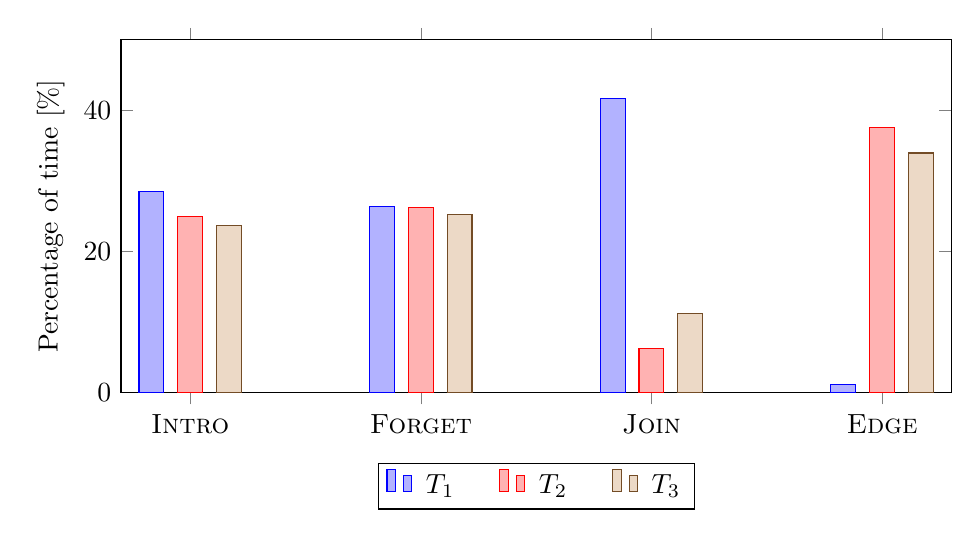
\begin{tikzpicture}
        \begin{axis}[
            width=\textwidth,
            height=0.5\textwidth,
            xtick=data,
            symbolic x coords={\textsc{Intro},\textsc{Forget},\textsc{Join},\textsc{Edge}},
            ylabel={Percentage of time [\%]},
            ymin=0,
            ymax=50,
            ybar=5pt, % configures `bar shift'
            legend style={at={(0.5,-0.2)},
            /tikz/every even column/.append style={column sep=0.5cm},
            /tikz/every odd column/.append style={column sep=0.1cm},
            anchor=north,legend columns=-1},
            bar width=9pt,
        ]
            \addplot coordinates {(\textsc{Intro}, 28.53) (\textsc{Forget}, 26.31)  (\textsc{Join}, 41.66)
            (\textsc{Edge}, 1.16)};

            \addplot coordinates {(\textsc{Intro}, 24.99) (\textsc{Forget}, 26.17)  (\textsc{Join}, 6.229)
            (\textsc{Edge}, 37.527)};

            \addplot coordinates {(\textsc{Intro}, 23.68) (\textsc{Forget}, 25.19)  (\textsc{Join}, 11.16)
            (\textsc{Edge}, 33.96)};

            \legend{$T_1$, $T_2$, $T_3$}
        \end{axis}
    \end{tikzpicture}
    \caption{Percentage of time spent on individual vertex types on tests from Example \ref{ex:tests}.}
    \label{fig:vertplot}
\end{figure}

For reference, we compare the absolute times to our older implementation using top-down formulas, as they are described
in Section \ref{sec:twdp}. Since this old version did not use the reduce method, for the measurement, we have turned
it off for the bottom-up version as well.

The results are displayed in Table \ref{tab:vertcomp}. It is notable, how fast is the bottom-up solution in comparison
with the top-down approach -- the older version needs over three seconds to compute the solution for $T_{low}$, while
for the new one, it only takes around 0.02 seconds. This comparison is not completely fair though, as there are several
optimizations in the bottom-up version that cannot be applied to the top-down approach, or just were not worth porting
to a version that does not support cut matrix reduction.

Still, the results clearly show that \textsc{Join} vertex computation completely dominate run time of a top-down
solution, which was constantly observed during early stages of development. This is also the source of largest
improvement brought by the new formulas, aside from enabling an efficient cut matrix usage.

\begin{table}[ht]

    \centering
    \begin{tabular}{ m{3cm} | m{1.5cm} m{1.5cm} m{1.5cm} m{1.5cm} }
        & \multicolumn{4}{c}{Time per vertex type} \\
        DP type & \textsc{Intro} & \textsc{Forget} & \textsc{Join} & \textsc{Edge} \\
        \midrule
        Top-down & 0.199\,s & 0.090\,s & 3.501\,s & 0.133\,s \\
        Bottom-up & 0.005\,s & 0.003\,s & 0.004\,s & 0.004\,s \\
    \end{tabular}

    \caption{Comparison of the top-down and the bottom-up solution on instance $T_{low}$ from Example \ref{ex:tests}.}
    \label{tab:vertcomp}
\end{table}

\subsection{Fast partition merging}
\label{sec:partmerge}

Following up on the description of \textsc{Join} vertex processing from the previous section, the algorithm spends
considerable amount of time on producing merges of two partitions, meaning we need to implement if efficiently.

We have implemented and compared two standard ways of merging graph components, modifying them for our use case of
partition merging, and being able to exclude cyclic results. Both ways are approximately equal in terms of asymptotic
time complexity (with a tiny added factor of an inverse Ackermann function in the Union-Find solution), so their
performance comparison comes down to constant factors, and efficiency of the early stop mechanism whenever a cycle is
detected.

\subsubsection*{Depth-first search merging}

Merging with a depth-first search is a straightforward solution, where we first create a graph representing each
element of $U$ with a vertex, and create an edge between each pair of vertices, that lie in the same component
within one of the merged partitions.

After the graph is built, we can run a standard depth-first search algorithm on each vertex, setting it to mark vertices
of the found component with a unique index whenever we start it from an unvisited vertex. After that, the merged
partition can be built by grouping vertices by their indices.

\subsubsection*{Union-find merging}

The union-find data structure (also commonly known as disjoint-set or DSU) is a classic way of dynamically keeping and
merging connected components in a graph, introduced in 1964 \cite{Galler1964}. It provides two operations over a fixed
set of (initially disjoint) elements $S$:

\begin{itemize}
    \item $union(a, b)$ where $a, b \in S$ -- Merges the components of $a$ and $b$. If $a$ and $b$ already belong
        to the same component, returns a \emph{false} boolean value, otherwise returns \emph{true}.

    \item $find(a)$, where $a \in S$ -- Returns a representative $r \in S$ of the component $a$ belongs to. This
        representative is guaranteed to be the same for all elements of this component, until any union operation is
        called.
\end{itemize}

It was proven in 1975 by Tarjan \cite{Tarjan1975}, that there is an implementation of the structure where both of these
operations have a worst case time complexity of $\mathcal{O}(\alpha(|S|))$, where $\alpha$ is an inverse Ackermann
function. As we are not going to consider partitions larger than 16 elements, the value of this function cannot be
higher than 4, essentially meaning each operation will take near-constant time to compute.

Using this data structure, merging partitions $P_1$ and $P_2$ of a subset $U$ can be implemented in a near-linear
time, as shown in Algorithm \ref{algo:unionfind}.

\begin{algorithm}
    \caption{Merging partitions with a union-find data structure}
    \label{algo:unionfind}
    \begin{algorithmic}[1]
        \State $uf \gets initUnionFind(U)$
        \State $repre_1 \gets \text{array of}\ |P_1|\ \text{empty elements}$
        \State $repre_2 \gets \text{array of}\ |P_2|\ \text{empty elements}$
        \For{$u \in U$}
            \State $c_1 \gets \text{component of}\ u\ \text{in}\ P_1$ 
            \State $c_2 \gets \text{component of}\ u\ \text{in}\ P_2$ 

            \If{$repre_1[c_1] = \text{empty}$}
                \State $repre_1[c_1] \gets u$
            \Else
                \If{$uf.union(repre_1[c_1], u) = false$}
                    \State \Return{\texttt{INVALID\_PARTITION}}
                \EndIf
            \EndIf

            \If{$repre_2[c_2] = \text{empty}$}
                \State $repre_2[c_2] \gets u$
            \Else
                \If{$uf.union(repre_2[c_2], u) = false$}
                    \State \Return{\texttt{INVALID\_PARTITION}}
                \EndIf
            \EndIf
        \EndFor

        \State \Return{components of $uf$ converted to a partition}
    \end{algorithmic}
\end{algorithm}

Note that we can perform an early stop to merging any time we try to merge an element with a component it already
belongs to. The solution for such partition would contain edges that provide redundant connectivity, meaning it cannot
be a part of an optimal final result.

\subsubsection*{Comparison}

We have tested both mergers on the PACE 2018 public dataset, only comparing the time performance of the JOIN operation.
From the results shown in Figure \ref{fig:partcomp}, it is apparent that the Union-find based merger performs better,
either because of its early stop rule, or due to the structure being more efficient than the edge checks in the
depth-first search.

\begin{figure}[ht]
    \centering
    \begin{tikzpicture}
        \begin{axis}[
            width=\textwidth,
            height=0.6\textwidth,
            xmin=1,
            xmax=28,
            ylabel={Time [s]},
            xlabel={Instance},
            ymin=0,
            ymax=1,
            legend style={at={(0.5,-0.2)},
            /tikz/every even column/.append style={column sep=0.5cm},
            /tikz/every odd column/.append style={column sep=0.1cm},
            anchor=north,legend columns=-1}
        ]
            \addplot[color=blue] table
            [x={a},y={b}]{plots/parts.pgf};

            \addplot[color=red] table
            [x={a},y={c}]{plots/parts.pgf};

            \legend{Union-find, DFS}
        \end{axis}
    \end{tikzpicture}
    \caption{Comparison of different partitions mergers on instances from PACE 2018 Track B input set.}
    \label{fig:partcomp}
\end{figure}

\subsection{Cut Matrix elimination using binary operations}

Reducing the number of stored partitions is a procedure that significantly speeds up computing of the dynamic
programming table, but takes a considerable amount of time itself. In this section, we will discuss its possible
optimization.

First, we can observe that the elimination is only guaranteed to reduce the number of considered partitions if their
count is higher than the number of cuts, which is $2^{|U|-1}$. If we have less partitions than that, we skip the whole
cut matrix construction and elimination.

Since the cut matrix only contains values 0 and 1, it is possible to speed up finding its basis by using bit sets, and
performing the elimination using binary operations. This will also help us reduce the size of the created matrix, saving
memory. Recall, that the modified Gaussian elimination which finds the cheapest basis can be performed as follows:

We iterate over each row of the cut matrix $\mathbb{C}$, with the rows being sorted by the weight of the solution for
their corresponding partition, and indexed in order of their ascending weight (columns can be indexed arbitrarily). While
considering row with index $r$, we find the column with the minimum index $c$, such that $\mathbb{C}[r][c] = 1$.

If there is no such column, the row is linearly dependent on rows with lesser weight, and we can thus discard its
corresponding partition. Otherwise, we will go through each row with index $r' > r$, and add row $r$ in module 2 to it
if $\mathbb{C}[r'][c] = 1$.

To optimize this, we can represent each row with a binary vector, implemented as an array of 64-bit integers. This
immediately results in 8 times smaller memory footprint, in comparison with storing a 1 byte variable for each value in
the matrix, and also means a much bigger portion of the matrix can fit in the CPU cache now.

Finding the left-most non-zero column can be done by finding the first non-zero integer in the row representation, then
calling a built-in function of the GCC compiler \cite{gcc} \texttt{\_\_builtin\_ffsll(i)}, which finds the position of
the first one in the binary representation of a 64-bit integer.

Row addition in module 2 can be simply implemented by the xor operation, applied on all pairs of row integers that
represent the same set of columns.

Both of these operations will use approximately 64 times less operations than the value-by-value searching and
adding we would have to do, if we have stored each value of $\mathbb{C}$ in a separate variable. This could be further
improved by making use of larger registers, or employing SIMD operations. However, measurements in Figure
\ref{fig:overprof} show that with these improvements, the elimination already takes negligible time in comparison with
the construction of the matrix itself, which needs to check whether a partition refines a cut for each value.

Unfortunately, the cut matrix construction times cannot be improved as easily, since the refinement check is not as
trivial as the xor operation or finding the most significant turned on bit. Caching the already computed rows for future
matrices comes to mind, but storing values for each encountered partition could significantly worsen the memory
complexity.

\section{Overall profiling data}

Finally, we will look at complete distribution of run times for individual steps of the algorithm, using inputs from Example
\ref{ex:tests}. The first four labels describe time spent on individual nice tree decomposition vertex types, the
description for remaining three is as follows:

\begin{itemize}
    \item \textsc{CM Gen}: Time spent to generate the cut matrix from the sorted list of partitions.

    \item \textsc{CM Red}: Time spent on elimination of the cut matrix.

    \item \textsc{CM Over}: All other operations associated with the cut matrix reduction, like reading and storing them
        to the dynamic programming cache.
\end{itemize}

As we can see in Figure \ref{fig:overprof}, with all optimizations applied, the largest amounts of time are actually
spent on generating matrices for the reduction, even though it is asymptotically less complex than the elimination
itself. This can be explained by the operations performed during eliminations being simpler, and sped up by the binary
vector usage, whereas during the matrix generation, we have to consider each element separately, and perform more
complex computation to find out if a partition refines cut.

The fraction of time spent on cut matrices drops for larger graphs, moving into tree decomposition vertex processing,
but it is still apparent that the largest optimization of this algorithm could be done if we found a way to create the
cut matrix more efficiently.

\begin{figure}
    \centering
    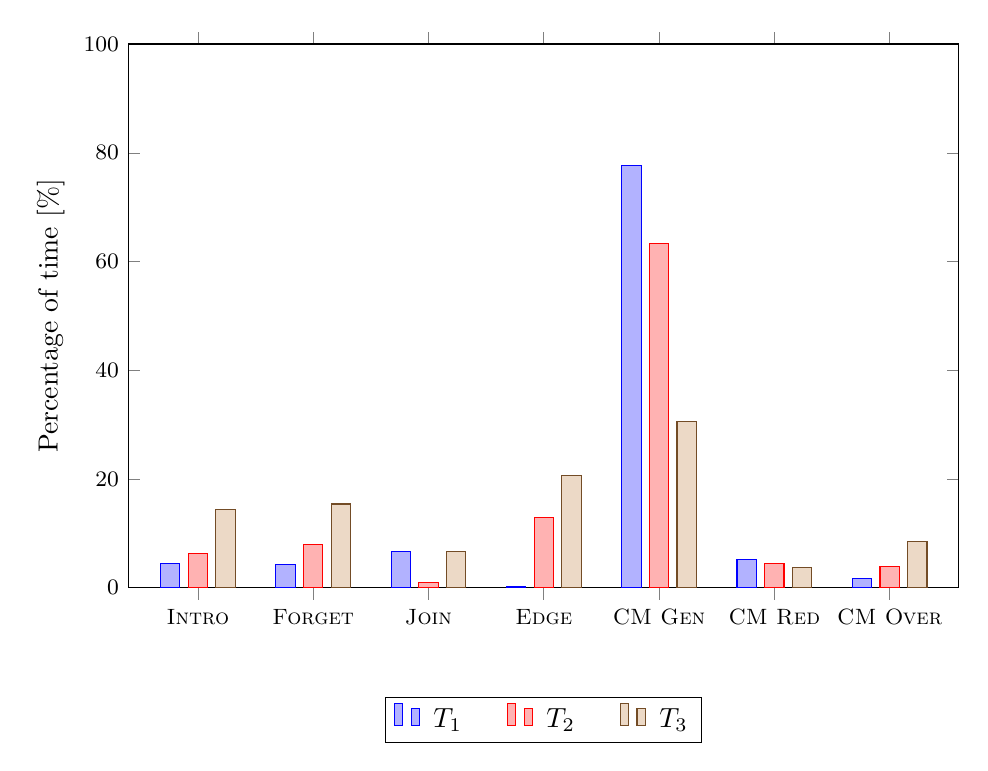
\begin{tikzpicture}
        \begin{axis}[
            width=\textwidth,
            height=0.7\textwidth,
            xtick=data,
            ticklabel style={font=\footnotesize},
            symbolic x coords={\textsc{Intro},\textsc{Forget},\textsc{Join},\textsc{Edge},\textsc{CM Gen},
            \textsc{CM Red},\textsc{CM Over}},
            ylabel={Percentage of time [\%]},
            ymin=0,
            ymax=100,
            ybar=3pt, % configures `bar shift'
            legend style={at={(0.5,-0.2)},
            /tikz/every even column/.append style={column sep=0.5cm},
            /tikz/every odd column/.append style={column sep=0.1cm},
            anchor=north,legend columns=-1},
            bar width=7pt,
        ]
            \addplot coordinates {(\textsc{Intro}, 4.43) (\textsc{Forget}, 4.21)  (\textsc{Join}, 6.64)
            (\textsc{Edge}, 0.15) (\textsc{CM Gen}, 77.6) (\textsc{CM Red}, 5.18) (\textsc{CM Over}, 1.79)};

            \addplot coordinates {(\textsc{Intro}, 6.31) (\textsc{Forget}, 7.96)  (\textsc{Join}, 0.98)
            (\textsc{Edge}, 12.92) (\textsc{CM Gen}, 63.34) (\textsc{CM Red}, 4.51) (\textsc{CM Over}, 3.98)};

            \addplot coordinates {(\textsc{Intro}, 14.43) (\textsc{Forget}, 15.42)  (\textsc{Join}, 6.76)
            (\textsc{Edge}, 20.65) (\textsc{CM Gen}, 30.57) (\textsc{CM Red}, 3.70) (\textsc{CM Over}, 8.48)};

            \legend{$T_1$, $T_2$, $T_3$}
        \end{axis}
    \end{tikzpicture}
    \caption{Percentage of time spent on individual algorithm parts, tested with inputs from Example \ref{ex:tests}.}
    \label{fig:overprof}
\end{figure}


% -----------------------------------------------------------------------------

\chapter{Comparison with other solutions}

We have submitted our implementation of algorithms described in the previous chapter into an international competition.
This way, it could be compared with various solutions made by participants from all over the world.

In this section, we will describe the challenge rules, testing and ranking methods, and results achieved in both
categories we have participated in.

\section{PACE challenge}

The Parameterized Algorithms and Computational Experiments Challenge (PACE) \cite{PaceWeb} is an annual programming
competition, focusing on parameterized versions of one or two different \NPH problems each year.

The first iteration of this challenge begun in Fall of 2015, we have participated in its third run, being announced on
November 14th, 2017, with the submission deadline on May 1st, 2018. The focus of this round was the \textsc{Steiner
Tree} problem, and it was divided into three tracks:

\begin{itemize}
    \item \textbf{A: Exact with few terminals} -- Required an exact solution, the inputs were tailored to test algorithms
        parameterized by the number of terminals.

    \item \textbf{B: Exact with low treewidth} -- Required an exact solution as well, the inputs included corresponding
        tree decomposition, and were scaled by the width of this decomposition, which was generally low.

    \item \textbf{C: Heuristic} -- Was rated by the weight of the solution, an optimal one was not required. Included
        various kinds of inputs, without focus on a specific parameter.
\end{itemize}

As our work revolves around exact algorithms, we have only participated in tracks A and B.

\section{Testing and ranking}
\label{sec:pacetest}

Aside from the problem description, challenge organizers provided 100 public problem instances for each track to use
for testing. To prevent optimizing for specific inputs, the solutions were tested on 100 similar private instances to
determine final rankings.

The input sets were gradually scaled by their tested parameter, and contained graphs of various types and sizes, sourced
from a mix of established benchmarks and real world problems \cite{PacePresentation}.

Consistent with our assumptions from previous chapters, all inputs for track B also contain their tree decompositions.
In some cases, these contained a flag marking that the decomposition is not guaranteed to have the minimum width, since
it was found by a heuristic. It opens a possibility of speeding up the solution by finding a better decomposition, but
since its finding was the topic of the PACE 2017 challenge, and the provided decomposition was found by its winner, we
have decided not to explore this option.

An online testing environment was also provided on the OPTIL.io platform \cite{OptilIo}, allowing full tests on public
instances once per 24 hours, and more frequent tests on a set of 10 instances with shorter time limits. Basically any
widely used programming language was supported both on the platform, and for the final submissions.

For the final test on private instances, the execution time limit for each instance was 30 minutes, and the sum of times
for all instances was otherwise unconstrained. Memory limits and hardware configuration were not officially announced,
but testing was likely carried out on the same OPTIL.io environment, as the one used for public testing.

The final ranking was decided by the number of solved instances, excluding any runs that ended by reaching time limit,
memory limit, or crashed due to a runtime error. Ties were resolved by the sum of execution times (though this notion
was not reflected in the final report). If an algorithm printed a wrong answer for any of the instances in one of the
exact tracks, it was disqualified regardless of other results in order to prohibit heuristic solutions.

\section{Results}

The results of the competition were presented at International Symposium on Parameterized and Exact Computation (IPEC
2018), and a detailed final report was published in its proceedings \cite{PaceReport}. We will briefly summarize
the results in this section, comparing our implementation to other submissions, and pointing out their approaches to the
problem.

\subsection{Track A: Number of terminals}

Based on our measurements from Chapter 4, we have not been able to optimize the Nederlof's algorithm to the extent where
it could surpass the performance of the Erickson-Monma-Veinott approach, meaning we have only used the latter
implementation.

Since the implementation was fairly straightforward, and only used basic preprocessing, we have finished at a shared 6th
place out of 12 teams. The full ranking presented in \cite{PaceReport} follows:

\begin{enumerate}
    \item
        \emph{(95/100 instances)} \textbf{Team wata\&sigma}: Yoichi Iwata and Takuto Shigemura, Japanese
        National Institute of Informatics and University of Tokyo
    \item
        \emph{(94/100 instances)} \textbf{Team Jagiellonian}: Krzysztof Maziarz and Adam Polak, Jagiellonian University
    \item
        \emph{(93/100 instances)} \textbf{Team reko}: Thorsten Koch and Daniel Rehfeldt, Zuse Institute Berlin and TU Berlin
    \item
        \emph{(92/100 instances)} \textbf{Team TUW}: Andre Schidler, Johannes Fichte, and Markus Hecher, TU Vienna
    \item
        \emph{(67/100 instances)} \textbf{Team UWarsaw}: Krzysztof Kiljan, Dominik Klemba, Marcin Mucha, Wojciech Nadara, Marcin
        Pilipczuk, Mateusz Radecki, and Michał Ziobro, University of Warsaw and Jagiellonian University
    \item
        \emph{(66/100 instances)} \textbf{Team Noname}: Suhas Thejaswi, Aalto University
        \addtocounter{enumi}{-1}
    \item
        \emph{(66/100 instances)} \textbf{Team FIT CTU in Prague}: Peter Mitura and Ondřej Suchý, Czech Technical University
        \addtocounter{enumi}{-1}
    \item
        \emph{(66/100 instances)} \textbf{Team TU Vienna}: Johannes Varga, TU Vienna
        \addtocounter{enumi}{2}
    \item
        \emph{(48/100 instances)} \textbf{Team SSPSPT}: Saket Saurabh, P. S. Srinivasan, and Prafullkumar Tale,
        the Institute Of Mathematical Sciences, HBNI, Chennai and the International Institute
        of Information Technology, Bangalore
    \item
        \emph{(69/100 instances, one incorrect)} \textbf{Team the65thbit}: Sharat Ibrahimpur, University of Waterloo
    \item
        \emph{(14/100 instances, several incorrect)} \textbf{Team PCCoders}: S. Vaishali and Rathna Subramanian, PSG
        College of Technology, Coimbatore
    \item
        \emph{(9/100 instances, several incorrect)} \textbf{Team Resilience}: R. Vijayaragunathan, N. S. Narayanaswamy,
        and Rajesh Pandian M., team Resilience from TCS Lab, Indian Institute of Technology, Madras
\end{enumerate}

Of the submitted solutions, all except the one on the third place used some version of the Erickson-Monma-Veinott or
Dreyfus-Wagner algorithm, with various tricks to preprocess the graph, and prune the state space in the dynamic
programming table. The solution by Team reko has used a mixed-integer programming solver SCIP, along with a number
of preprocessing methods to reduce the complexity of an instance.

\subsection{Track B: Treewidth}

In Track B, we have submitted the optimized rank-based algorithm described in Section \ref{sec:twimpl}, with a
possibility to switch to our Track A implementation if the number of terminals is below 14, or the treewidth is higher
than 16. In the final results, our implementation has achieved a shared fourth place with 52 solved instances out of
100, and has been referred to as ``the fastest of the competition on average'' in its track. The full ranking presented
in \cite{PaceReport} follows:

\begin{enumerate}
    \item \emph{(92/100 instances)} \textbf{Team reko}: Thorsten Koch and Daniel Rehfeldtteam, Zuse Institute
        Berlin and TU Berlin
    \item \emph{(77/100 instances)} \textbf{Team wata\&sigma}: Yoichi Iwata and Takuto Shigemura, Japanese National
        Institute of Informatics and the University of Tokyo
    \item \emph{(58/100 instances)} \textbf{Team Tom}: Tom van der Zanden, Utrecht University
    \item \emph{(52/100 instances)} \textbf{Team FIT CTU in Prague}: Peter Mitura and Ondřej Suchý, Czech Technical
        University
        \addtocounter{enumi}{-1}
    \item \emph{(52/100 instances)} \textbf{Team Yasu}: Yasuaki Kobayashi, Kyoto University
        \addtocounter{enumi}{1}
    \item \emph{(49/100 instances)} \textbf{Team CBGfinder}: Akio Fujiyoshi, Ibaraki University
    \item \emph{(33/100 instances)} \textbf{Team UWarsaw}: Krzysztof Kiljan, Dominik Klemba, Marcin Mucha, Wojciech
        Nadara, Marcin Pilipczuk, Mateusz Radecki, and Michał Ziobro, University of Warsaw and Jagiellonian University
        \addtocounter{enumi}{-1}
    \item \emph{(33/100 instances)} \textbf{Team lapo}: Dilson Guimarães, Guilherme Gomes, João Gonçalves, and Vinícius dos
        Santos, LAPO-UFMG
        \addtocounter{enumi}{1}
\end{enumerate}


Interestingly, the first two entries mostly did not rely on a solution that was parameterized by treewidth. The winning
implementation from team reko utilized the same solution as in Track A, utilizing a mixed-integer programming solver
SCIP, already mentioned in the previous section.

The second team wata\&sigma has re-used their solution parameterized by the number of terminals, with which they have
won in the Track A. It utilized a standard Erickson-Monma-Veinott algorithm with additional pruning rules, that
allowed it to solve many instances in Track B that did not have extremely high number of terminals as well. For inputs
with low treewidth, they have also included a simple implementation of the classical dynamic programming solution with
$\mathcal{O}^*(t^{\mathcal{O}(t)})$ complexity, improving their results in the first half of instances.

The first implementation, that (almost) purely used a solution parameterized by treewidth ended third, made by Tom van
der Zanden. It uses the cut matrix approach, utilizing various optimization techniques, partially referenced from the
work of L.W. van der Graaff \cite{Graaff2015}.

In comparison with our implementation, it uses many optimizations similar to ours, as in cut matrix binary operations,
backtracking table representation and partition merging. On the top, it introduces improvements like faster processing
of multiple \textsc{Introduce Edge} vertices, nice tree decomposition preprocessing, more sophisticated rules for reduce
method launching, and more efficient cut matrix generation. It, however, uses byte arrays to represent partitions, meaning
our solution should be able to query the dynamic programming table more efficiently.

This, along with the programming language choice (Tom van der Zanden's solution utilizes C\#) can explain why our
solution processes smaller instances faster, but fell short on larger inputs. In Figures \ref{fig:tomcomp} and
\ref{fig:tomsmallcomp}, we show a comparison of run times for both solutions, done with our testing setup described in
Section \ref{sec:setup} on public instances. Our algorithm truly performs faster on smaller instances, but starts to
exhibit higher spikes in run time than the higher placed solution on larger instances.

In Table \ref{tab:trackb}, a full listing of final results for first five teams is displayed, taken from OPTIL.io
\cite{OptilIo} leaderboard. Note that the result descriptions use standard competitive programming abbreviations, which
are explained in the Acronyms section at the end of the thesis. Some instances, where all teams received the AC status,
were omitted for conciseness.

The results show, that while ignoring the tree decomposition enabled the first two solutions to solve many instances
where treewidth parameterized algorithms were not feasible, there were instances with lower treewidth that were only
solved by rank-based algorithms, and these solutions were more consistent in overall for inputs with treewidth up to 14
(around instance number 50).

\begin{figure}[ht]
    \centering
    \begin{tikzpicture}
        \begin{axis}[
            width=\textwidth,
            height=0.6\textwidth,
            xmin=1,
            xmax=25,
            ylabel={Time [s]},
            xlabel={Instance},
            ymin=0,
            ymax=10,
            legend style={at={(0.5,-0.2)},
            /tikz/every even column/.append style={column sep=0.5cm},
            /tikz/every odd column/.append style={column sep=0.1cm},
            anchor=north,legend columns=-1}
        ]
            \addplot[color=blue] table
            [x={a},y={b}]{plots/perf_comp.pgf};

            \addplot[color=red] table
            [x={a},y={c}]{plots/perf_comp.pgf};

            \legend{Team FIT CTU, Team Tom}
        \end{axis}
    \end{tikzpicture}
    \caption{Comparison of Track B solution run times on smaller public instances, with the testing setup described in
    Section \ref{sec:setup}.}
    \label{fig:tomsmallcomp}
\end{figure}

\begin{figure}[ht]
    \centering
    \begin{tikzpicture}
        \begin{axis}[
            width=\textwidth,
            height=0.6\textwidth,
            xmin=25,
            xmax=37,
            ylabel={Time [s]},
            xlabel={Instance},
            ymin=0,
            ymax=50,
            legend style={at={(0.5,-0.2)},
            /tikz/every even column/.append style={column sep=0.5cm},
            /tikz/every odd column/.append style={column sep=0.1cm},
            anchor=north,legend columns=-1}
        ]
            \addplot[color=blue] table
            [x={a},y={b}]{plots/perf_comp.pgf};

            \addplot[color=red] table
            [x={a},y={c}]{plots/perf_comp.pgf};

            \legend{Team FIT CTU, Team Tom}
        \end{axis}
    \end{tikzpicture}
    \caption{Comparison of Track B solution run times on larger public instances, with the testing setup described in
    Section \ref{sec:setup}.}
    \label{fig:tomcomp}
\end{figure}

\begin{table}[ht]
    \tiny
    \centering
    \begin{tabular}{ m{1cm} | m{1.5cm} m{1.5cm} m{1.5cm} m{1.5cm} m{1.5cm} }
        \toprule
        & \multicolumn{5}{c}{Team name} \\
        Instance & reko & wata\&sigma & Tom & FIT CTU & yasu \\
        \midrule
        % 1 & \textcolor{ForestGreen}{AC} & \textcolor{ForestGreen}{AC} & \textcolor{ForestGreen}{AC} & \textcolor{ForestGreen}{AC} & \textcolor{ForestGreen}{AC} \\
        % 2 & \textcolor{ForestGreen}{AC} & \textcolor{ForestGreen}{AC} & \textcolor{ForestGreen}{AC} & \textcolor{ForestGreen}{AC} & \textcolor{ForestGreen}{AC} \\
        % 3 & \textcolor{ForestGreen}{AC} & \textcolor{ForestGreen}{AC} & \textcolor{ForestGreen}{AC} & \textcolor{ForestGreen}{AC} & \textcolor{ForestGreen}{AC} \\
        % 4 & \textcolor{ForestGreen}{AC} & \textcolor{ForestGreen}{AC} & \textcolor{ForestGreen}{AC} & \textcolor{ForestGreen}{AC} & \textcolor{ForestGreen}{AC} \\
        % 5 & \textcolor{ForestGreen}{AC} & \textcolor{ForestGreen}{AC} & \textcolor{ForestGreen}{AC} & \textcolor{ForestGreen}{AC} & \textcolor{ForestGreen}{AC} \\
        % 6 & \textcolor{ForestGreen}{AC} & \textcolor{ForestGreen}{AC} & \textcolor{ForestGreen}{AC} & \textcolor{ForestGreen}{AC} & \textcolor{ForestGreen}{AC} \\
        % 7 & \textcolor{ForestGreen}{AC} & \textcolor{ForestGreen}{AC} & \textcolor{ForestGreen}{AC} & \textcolor{ForestGreen}{AC} & \textcolor{ForestGreen}{AC} \\
        % 8 & \textcolor{ForestGreen}{AC} & \textcolor{ForestGreen}{AC} & \textcolor{ForestGreen}{AC} & \textcolor{ForestGreen}{AC} & \textcolor{ForestGreen}{AC} \\
        % 9 & \textcolor{ForestGreen}{AC} & \textcolor{ForestGreen}{AC} & \textcolor{ForestGreen}{AC} & \textcolor{ForestGreen}{AC} & \textcolor{ForestGreen}{AC} \\
        % 10 & \textcolor{ForestGreen}{AC} & \textcolor{ForestGreen}{AC} & \textcolor{ForestGreen}{AC} & \textcolor{ForestGreen}{AC} & \textcolor{ForestGreen}{AC} \\
        % 11 & \textcolor{ForestGreen}{AC} & \textcolor{ForestGreen}{AC} & \textcolor{ForestGreen}{AC} & \textcolor{ForestGreen}{AC} & \textcolor{ForestGreen}{AC} \\
        % 12 & \textcolor{ForestGreen}{AC} & \textcolor{ForestGreen}{AC} & \textcolor{ForestGreen}{AC} & \textcolor{ForestGreen}{AC} & \textcolor{ForestGreen}{AC} \\
        13 & \textcolor{ForestGreen}{AC} & \textcolor{ForestGreen}{AC} & \textcolor{ForestGreen}{AC} & \textcolor{ForestGreen}{AC} & \textcolor{Red}{RTE} \\
        % 14 & \textcolor{ForestGreen}{AC} & \textcolor{ForestGreen}{AC} & \textcolor{ForestGreen}{AC} & \textcolor{ForestGreen}{AC} & \textcolor{ForestGreen}{AC} \\
        % 15 & \textcolor{ForestGreen}{AC} & \textcolor{ForestGreen}{AC} & \textcolor{ForestGreen}{AC} & \textcolor{ForestGreen}{AC} & \textcolor{ForestGreen}{AC} \\
        % 16 & \textcolor{ForestGreen}{AC} & \textcolor{ForestGreen}{AC} & \textcolor{ForestGreen}{AC} & \textcolor{ForestGreen}{AC} & \textcolor{ForestGreen}{AC} \\
        % 17 & \textcolor{ForestGreen}{AC} & \textcolor{ForestGreen}{AC} & \textcolor{ForestGreen}{AC} & \textcolor{ForestGreen}{AC} & \textcolor{ForestGreen}{AC} \\
        % 18 & \textcolor{ForestGreen}{AC} & \textcolor{ForestGreen}{AC} & \textcolor{ForestGreen}{AC} & \textcolor{ForestGreen}{AC} & \textcolor{ForestGreen}{AC} \\
        % 19 & \textcolor{ForestGreen}{AC} & \textcolor{ForestGreen}{AC} & \textcolor{ForestGreen}{AC} & \textcolor{ForestGreen}{AC} & \textcolor{ForestGreen}{AC} \\
        % 20 & \textcolor{ForestGreen}{AC} & \textcolor{ForestGreen}{AC} & \textcolor{ForestGreen}{AC} & \textcolor{ForestGreen}{AC} & \textcolor{ForestGreen}{AC} \\
        % 21 & \textcolor{ForestGreen}{AC} & \textcolor{ForestGreen}{AC} & \textcolor{ForestGreen}{AC} & \textcolor{ForestGreen}{AC} & \textcolor{ForestGreen}{AC} \\
        % 22 & \textcolor{ForestGreen}{AC} & \textcolor{ForestGreen}{AC} & \textcolor{ForestGreen}{AC} & \textcolor{ForestGreen}{AC} & \textcolor{ForestGreen}{AC} \\
        % 23 & \textcolor{ForestGreen}{AC} & \textcolor{ForestGreen}{AC} & \textcolor{ForestGreen}{AC} & \textcolor{ForestGreen}{AC} & \textcolor{ForestGreen}{AC} \\
        % 24 & \textcolor{ForestGreen}{AC} & \textcolor{ForestGreen}{AC} & \textcolor{ForestGreen}{AC} & \textcolor{ForestGreen}{AC} & \textcolor{ForestGreen}{AC} \\
        % 25 & \textcolor{ForestGreen}{AC} & \textcolor{ForestGreen}{AC} & \textcolor{ForestGreen}{AC} & \textcolor{ForestGreen}{AC} & \textcolor{ForestGreen}{AC} \\
        26 & \textcolor{Red}{TLE} & \textcolor{Red}{MLE} & \textcolor{ForestGreen}{AC} & \textcolor{ForestGreen}{AC} & \textcolor{Red}{RTE} \\
        % 27 & \textcolor{ForestGreen}{AC} & \textcolor{ForestGreen}{AC} & \textcolor{ForestGreen}{AC} & \textcolor{ForestGreen}{AC} & \textcolor{ForestGreen}{AC} \\
        % 28 & \textcolor{ForestGreen}{AC} & \textcolor{ForestGreen}{AC} & \textcolor{ForestGreen}{AC} & \textcolor{ForestGreen}{AC} & \textcolor{ForestGreen}{AC} \\
        % 29 & \textcolor{ForestGreen}{AC} & \textcolor{ForestGreen}{AC} & \textcolor{ForestGreen}{AC} & \textcolor{ForestGreen}{AC} & \textcolor{ForestGreen}{AC} \\
        % 30 & \textcolor{ForestGreen}{AC} & \textcolor{ForestGreen}{AC} & \textcolor{ForestGreen}{AC} & \textcolor{ForestGreen}{AC} & \textcolor{ForestGreen}{AC} \\
        % 31 & \textcolor{ForestGreen}{AC} & \textcolor{ForestGreen}{AC} & \textcolor{ForestGreen}{AC} & \textcolor{ForestGreen}{AC} & \textcolor{ForestGreen}{AC} \\
        % 32 & \textcolor{ForestGreen}{AC} & \textcolor{ForestGreen}{AC} & \textcolor{ForestGreen}{AC} & \textcolor{ForestGreen}{AC} & \textcolor{ForestGreen}{AC} \\
        33 & \textcolor{ForestGreen}{AC} & \textcolor{Red}{MLE} & \textcolor{ForestGreen}{AC} & \textcolor{ForestGreen}{AC} & \textcolor{ForestGreen}{AC} \\
        % 34 & \textcolor{ForestGreen}{AC} & \textcolor{ForestGreen}{AC} & \textcolor{ForestGreen}{AC} & \textcolor{ForestGreen}{AC} & \textcolor{ForestGreen}{AC} \\
        35 & \textcolor{ForestGreen}{AC} & \textcolor{Red}{MLE} & \textcolor{ForestGreen}{AC} & \textcolor{ForestGreen}{AC} & \textcolor{ForestGreen}{AC} \\
        % 36 & \textcolor{ForestGreen}{AC} & \textcolor{ForestGreen}{AC} & \textcolor{ForestGreen}{AC} & \textcolor{ForestGreen}{AC} & \textcolor{ForestGreen}{AC} \\
        % 37 & \textcolor{ForestGreen}{AC} & \textcolor{ForestGreen}{AC} & \textcolor{ForestGreen}{AC} & \textcolor{ForestGreen}{AC} & \textcolor{ForestGreen}{AC} \\
        38 & \textcolor{Red}{TLE} & \textcolor{Red}{MLE} & \textcolor{ForestGreen}{AC} & \textcolor{ForestGreen}{AC} & \textcolor{ForestGreen}{AC} \\
        39 & \textcolor{Red}{TLE} & \textcolor{Red}{MLE} & \textcolor{ForestGreen}{AC} & \textcolor{Red}{MLE} & \textcolor{Red}{TLE} \\
        % 40 & \textcolor{ForestGreen}{AC} & \textcolor{ForestGreen}{AC} & \textcolor{ForestGreen}{AC} & \textcolor{ForestGreen}{AC} & \textcolor{ForestGreen}{AC} \\
        % 41 & \textcolor{ForestGreen}{AC} & \textcolor{ForestGreen}{AC} & \textcolor{ForestGreen}{AC} & \textcolor{ForestGreen}{AC} & \textcolor{ForestGreen}{AC} \\
        % 42 & \textcolor{ForestGreen}{AC} & \textcolor{ForestGreen}{AC} & \textcolor{ForestGreen}{AC} & \textcolor{ForestGreen}{AC} & \textcolor{ForestGreen}{AC} \\
        43 & \textcolor{ForestGreen}{AC} & \textcolor{Red}{MLE} & \textcolor{ForestGreen}{AC} & \textcolor{ForestGreen}{AC} & \textcolor{ForestGreen}{AC} \\
        44 & \textcolor{ForestGreen}{AC} & \textcolor{Red}{MLE} & \textcolor{ForestGreen}{AC} & \textcolor{ForestGreen}{AC} & \textcolor{ForestGreen}{AC} \\
        % 45 & \textcolor{ForestGreen}{AC} & \textcolor{ForestGreen}{AC} & \textcolor{ForestGreen}{AC} & \textcolor{ForestGreen}{AC} & \textcolor{ForestGreen}{AC} \\
        % 46 & \textcolor{ForestGreen}{AC} & \textcolor{ForestGreen}{AC} & \textcolor{ForestGreen}{AC} & \textcolor{ForestGreen}{AC} & \textcolor{ForestGreen}{AC} \\
        % 47 & \textcolor{ForestGreen}{AC} & \textcolor{ForestGreen}{AC} & \textcolor{ForestGreen}{AC} & \textcolor{ForestGreen}{AC} & \textcolor{ForestGreen}{AC} \\
        48 & \textcolor{ForestGreen}{AC} & \textcolor{Red}{MLE} & \textcolor{ForestGreen}{AC} & \textcolor{ForestGreen}{AC} & \textcolor{ForestGreen}{AC} \\
        % 49 & \textcolor{ForestGreen}{AC} & \textcolor{ForestGreen}{AC} & \textcolor{ForestGreen}{AC} & \textcolor{ForestGreen}{AC} & \textcolor{ForestGreen}{AC} \\
        50 & \textcolor{ForestGreen}{AC} & \textcolor{Red}{MLE} & \textcolor{ForestGreen}{AC} & \textcolor{ForestGreen}{AC} & \textcolor{ForestGreen}{AC} \\
        51 & \textcolor{ForestGreen}{AC} & \textcolor{ForestGreen}{AC} & \textcolor{ForestGreen}{AC} & \textcolor{Red}{MLE} & \textcolor{ForestGreen}{AC} \\
        52 & \textcolor{ForestGreen}{AC} & \textcolor{ForestGreen}{AC} & \textcolor{ForestGreen}{AC} & \textcolor{Red}{TLE} & \textcolor{Red}{TLE} \\
        53 & \textcolor{ForestGreen}{AC} & \textcolor{Red}{MLE} & \textcolor{ForestGreen}{AC} & \textcolor{Red}{MLE} & \textcolor{ForestGreen}{AC} \\
        54 & \textcolor{ForestGreen}{AC} & \textcolor{ForestGreen}{AC} & \textcolor{Red}{MLE} & \textcolor{Red}{TLE} & \textcolor{Red}{TLE} \\
        55 & \textcolor{ForestGreen}{AC} & \textcolor{Red}{MLE} & \textcolor{ForestGreen}{AC} & \textcolor{Red}{RTE} & \textcolor{Red}{TLE} \\
        56 & \textcolor{ForestGreen}{AC} & \textcolor{Red}{MLE} & \textcolor{Red}{MLE} & \textcolor{Red}{MLE} & \textcolor{Red}{TLE} \\
        57 & \textcolor{ForestGreen}{AC} & \textcolor{ForestGreen}{AC} & \textcolor{ForestGreen}{AC} & \textcolor{ForestGreen}{AC} & \textcolor{ForestGreen}{AC} \\
        58 & \textcolor{ForestGreen}{AC} & \textcolor{ForestGreen}{AC} & \textcolor{Red}{MLE} & \textcolor{Red}{MLE} & \textcolor{Red}{RTE} \\
        59 & \textcolor{ForestGreen}{AC} & \textcolor{ForestGreen}{AC} & \textcolor{Red}{TLE} & \textcolor{Red}{MLE} & \textcolor{Red}{RTE} \\
        60 & \textcolor{ForestGreen}{AC} & \textcolor{ForestGreen}{AC} & \textcolor{Red}{MLE} & \textcolor{Red}{RTE} & \textcolor{Red}{RTE} \\
        61 & \textcolor{ForestGreen}{AC} & \textcolor{Red}{MLE} & \textcolor{Red}{TLE} & \textcolor{Red}{RTE} & \textcolor{Red}{RTE} \\
        62 & \textcolor{Red}{TLE} & \textcolor{Red}{MLE} & \textcolor{Red}{TLE} & \textcolor{Red}{RTE} & \textcolor{Red}{RTE} \\
        63 & \textcolor{ForestGreen}{AC} & \textcolor{ForestGreen}{AC} & \textcolor{Red}{MLE} & \textcolor{Red}{MLE} & \textcolor{Red}{TLE} \\
        64 & \textcolor{ForestGreen}{AC} & \textcolor{ForestGreen}{AC} & \textcolor{ForestGreen}{AC} & \textcolor{ForestGreen}{AC} & \textcolor{ForestGreen}{AC} \\
        65 & \textcolor{ForestGreen}{AC} & \textcolor{ForestGreen}{AC} & \textcolor{Red}{MLE} & \textcolor{Red}{RTE} & \textcolor{Red}{RTE} \\
        66 & \textcolor{ForestGreen}{AC} & \textcolor{ForestGreen}{AC} & \textcolor{Red}{MLE} & \textcolor{Red}{RTE} & \textcolor{Red}{RTE} \\
        67 & \textcolor{ForestGreen}{AC} & \textcolor{Red}{MLE} & \textcolor{Red}{TLE} & \textcolor{Red}{MLE} & \textcolor{Red}{RTE} \\
        68 & \textcolor{ForestGreen}{AC} & \textcolor{Red}{MLE} & \textcolor{Red}{TLE} & \textcolor{Red}{RTE} & \textcolor{Red}{RTE} \\
        69 & \textcolor{ForestGreen}{AC} & \textcolor{Red}{MLE} & \textcolor{Red}{MLE} & \textcolor{Red}{MLE} & \textcolor{Red}{RTE} \\
        70 & \textcolor{ForestGreen}{AC} & \textcolor{ForestGreen}{AC} & \textcolor{Red}{MLE} & \textcolor{Red}{MLE} & \textcolor{Red}{TLE} \\
        71 & \textcolor{ForestGreen}{AC} & \textcolor{ForestGreen}{AC} & \textcolor{Red}{MLE} & \textcolor{Red}{MLE} & \textcolor{Red}{RTE} \\
        72 & \textcolor{ForestGreen}{AC} & \textcolor{ForestGreen}{AC} & \textcolor{Red}{MLE} & \textcolor{Red}{RTE} & \textcolor{Red}{RTE} \\
        73 & \textcolor{ForestGreen}{AC} & \textcolor{ForestGreen}{AC} & \textcolor{Red}{MLE} & \textcolor{Red}{RTE} & \textcolor{Red}{RTE} \\
        74 & \textcolor{ForestGreen}{AC} & \textcolor{ForestGreen}{AC} & \textcolor{Red}{MLE} & \textcolor{Red}{MLE} & \textcolor{Red}{RTE} \\
        75 & \textcolor{ForestGreen}{AC} & \textcolor{ForestGreen}{AC} & \textcolor{Red}{TLE} & \textcolor{Red}{RTE} & \textcolor{Red}{RTE} \\
        76 & \textcolor{ForestGreen}{AC} & \textcolor{ForestGreen}{AC} & \textcolor{Red}{MLE} & \textcolor{Red}{MLE} & \textcolor{Red}{RTE} \\
        77 & \textcolor{ForestGreen}{AC} & \textcolor{ForestGreen}{AC} & \textcolor{Red}{MLE} & \textcolor{Red}{MLE} & \textcolor{Red}{RTE} \\
        78 & \textcolor{ForestGreen}{AC} & \textcolor{ForestGreen}{AC} & \textcolor{Red}{MLE} & \textcolor{Red}{RTE} & \textcolor{Red}{RTE} \\
        79 & \textcolor{ForestGreen}{AC} & \textcolor{Red}{MLE} & \textcolor{Red}{TLE} & \textcolor{Red}{RTE} & \textcolor{Red}{RTE} \\
        80 & \textcolor{ForestGreen}{AC} & \textcolor{Red}{MLE} & \textcolor{ForestGreen}{AC} & \textcolor{Red}{MLE} & \textcolor{Red}{RTE} \\
        81 & \textcolor{ForestGreen}{AC} & \textcolor{ForestGreen}{AC} & \textcolor{Red}{TLE} & \textcolor{Red}{RTE} & \textcolor{Red}{RTE} \\
        82 & \textcolor{ForestGreen}{AC} & \textcolor{ForestGreen}{AC} & \textcolor{Red}{MLE} & \textcolor{Red}{MLE} & \textcolor{Red}{RTE} \\
        83 & \textcolor{ForestGreen}{AC} & \textcolor{ForestGreen}{AC} & \textcolor{Red}{MLE} & \textcolor{Red}{MLE} & \textcolor{Red}{TLE} \\
        84 & \textcolor{ForestGreen}{AC} & \textcolor{Red}{MLE} & \textcolor{Red}{MLE} & \textcolor{Red}{RTE} & \textcolor{Red}{RTE} \\
        85 & \textcolor{ForestGreen}{AC} & \textcolor{ForestGreen}{AC} & \textcolor{Red}{TLE} & \textcolor{Red}{MLE} & \textcolor{Red}{TLE} \\
        86 & \textcolor{ForestGreen}{AC} & \textcolor{ForestGreen}{AC} & \textcolor{Red}{MLE} & \textcolor{Red}{RTE} & \textcolor{Red}{RTE} \\
        87 & \textcolor{ForestGreen}{AC} & \textcolor{ForestGreen}{AC} & \textcolor{Red}{MLE} & \textcolor{Red}{RTE} & \textcolor{Red}{RTE} \\
        88 & \textcolor{ForestGreen}{AC} & \textcolor{ForestGreen}{AC} & \textcolor{ForestGreen}{AC} & \textcolor{ForestGreen}{AC} & \textcolor{ForestGreen}{AC} \\
        89 & \textcolor{ForestGreen}{AC} & \textcolor{Red}{MLE} & \textcolor{Red}{TLE} & \textcolor{Red}{MLE} & \textcolor{Red}{RTE} \\
        90 & \textcolor{ForestGreen}{AC} & \textcolor{ForestGreen}{AC} & \textcolor{Red}{MLE} & \textcolor{Red}{RTE} & \textcolor{Red}{RTE} \\
        91 & \textcolor{ForestGreen}{AC} & \textcolor{ForestGreen}{AC} & \textcolor{Red}{MLE} & \textcolor{Red}{MLE} & \textcolor{Red}{RTE} \\
        92 & \textcolor{ForestGreen}{AC} & \textcolor{ForestGreen}{AC} & \textcolor{Red}{TLE} & \textcolor{Red}{RTE} & \textcolor{Red}{RTE} \\
        93 & \textcolor{Red}{TLE} & \textcolor{Red}{MLE} & \textcolor{Red}{TLE} & \textcolor{Red}{RTE} & \textcolor{Red}{RTE} \\
        94 & \textcolor{ForestGreen}{AC} & \textcolor{ForestGreen}{AC} & \textcolor{Red}{MLE} & \textcolor{Red}{RTE} & \textcolor{Red}{RTE} \\
        95 & \textcolor{Red}{TLE} & \textcolor{ForestGreen}{AC} & \textcolor{Red}{TLE} & \textcolor{Red}{RTE} & \textcolor{Red}{RTE} \\
        96 & \textcolor{ForestGreen}{AC} & \textcolor{ForestGreen}{AC} & \textcolor{Red}{MLE} & \textcolor{Red}{RTE} & \textcolor{Red}{RTE} \\
        97 & \textcolor{ForestGreen}{AC} & \textcolor{ForestGreen}{AC} & \textcolor{Red}{RTE} & \textcolor{Red}{RTE} & \textcolor{Red}{RTE} \\
        98 & \textcolor{ForestGreen}{AC} & \textcolor{ForestGreen}{AC} & \textcolor{Red}{TLE} & \textcolor{Red}{MLE} & \textcolor{Red}{TLE} \\
        99 & \textcolor{Red}{TLE} & \textcolor{Red}{TLE} & \textcolor{Red}{RTE} & \textcolor{Red}{MLE} & \textcolor{Red}{RTE} \\
        100 & \textcolor{Red}{TLE} & \textcolor{ForestGreen}{AC} & \textcolor{Red}{RTE} & \textcolor{Red}{RTE} & \textcolor{Red}{RTE} \\
        \bottomrule
    \end{tabular}

    \caption{Final results on Track B private instances for first five teams, without some cases where all teams
    succeeded.}
    \label{tab:trackb}
\end{table}

\setsecnumdepth{part}
\chapter{Conclusion}

We have successfully described and implemented several parameterized algorithms the \textsc{Steiner Tree} problem, tested and applied
various optimizations to them, and sent the end product to compete in the PACE 2018 challenge.

The main result is an implementation of the treewidth parameterized solution for Track B of the challenge, that reached
a shared 4th place in the overall ranking, was the second best performing algorithm using the rank-based approach if we
take total run times into account, and was referred to as the fastest solution in Track B on average.

In conclusion, the created solution for \textsc{Steiner Tree} problem instances with low treewidth has fared well in an
international competition, and seems to be a viable for instances with very low values of the parameter, where it
surpasses other alternatives.

As for future work, it would be surely interesting to combine improvements from various algorithms in Track B, and
create even faster implementation of the rank-based solution. Merging approaches from several tracks, and
choosing the best parameterization based on the input to create a general \textsc{Steiner Tree} problem solver could also
be beneficial.

In Track A of the competition, we have mostly seen variations on the classical Erickson-Monma-Veinott algorithm,
augmented with various preprocessing and pruning rules, with the sole exception of the MIP solver based solution.
Nederlof's inclusion-exclusion based algorithm has a potential to surpass them with its better exponential factor in
time complexity, but it is significantly slowed down by large polynomial factors associated with weighted, optimization
variant of the problem. 

Finding a way to reduce these, or exploring the possibility of finding a different approach with $\mathcal{O}^*(2^k)$
time complexity could improve the current results, especially when combined with preprocessing techniques shown by
submissions in the PACE challenge.

\medskip

All implementations, as they were submitted to the challenge, and included in the attached media, are available at
\url{https://github.com/PMitura/master-thesis}.

\bibliographystyle{alpha}
\bibliography{bibliography}

\setsecnumdepth{all}
\appendix

\chapter{Acronyms}
\begin{description}
    \item[AC] Accepted
    \item[CPU] Central Processing Unit
    \item[MIP] Mixed-Integer Programming
    \item[MLE] Memory Limit Exceeded
    \item[PACE] Parameterized Algorithms and Computational Experiments
    \item[RAM] Random Access Memory
    \item[RTE] Runtime Error
    \item[SIMD] Single Instruction, Multiple Data
    \item[TLE] Time Limit Exceeded
    \item[WA] Wrong Answer
\end{description}


\chapter{Contents of enclosed SD card}


\begin{figure}
    All of the SD card contents are also available at 
    \url{https://github.com/PMitura/master-thesis}.
    \bigskip
    \dirtree{%
        .1 impl\DTcomment{Solution sent to the PACE challenge}.
        .2 src/\DTcomment{Source codes of the implementation}.
        .2 CMakeLists.txt\DTcomment{CMake build file}.
        .2 README.md\DTcomment{Installation and usage instructions}.
        .1 legacy\_impl\DTcomment{Legacy runner of Track A candidate solutions}.
        .2 legacy\_impl.cpp\DTcomment{Legacy implementation of Track A candidates}.
        .2 Makefile\DTcomment{Make build file}.
        .2 README.md\DTcomment{Installation and usage instructions}.
        .1 thesis/\DTcomment{Source files of this thesis}.
    }
\end{figure}

\end{document}
